\chapter{Simulations}\label{c:simulations}

This chapter details the attempts at reproducing micropillar tensile tests on single crystal Ni, performed by Alan Xu and Dhriti Bhattacharyya at ANSTO Sydney.

\section{Methodology}

\subsection{Experimental setup}
\label{ss:experimentalSetup}

In total, eight loading tests were carried out.
\begin{enumerate}
    \item Tensile loading in $\langle 1\, 0\, 0 \rangle$:
          \begin{enumerate}
              \item Two tests with a loading rate of $\SI{5}{\nano\metre\per\second}$.
              \item Two tests with a loading rate of $\SI{500}{\nano\metre\per\second}$.
          \end{enumerate}
    \item Tensile loading in $\langle 1\, 1\, 0 \rangle$:
          \begin{enumerate}
              \item Two tests with a loading rate of $\SI{5}{\nano\metre\per\second}$.
              \item Two tests with a loading rate of $\SI{500}{\nano\metre\per\second}$.
          \end{enumerate}
\end{enumerate}

The cross-section of the micropillars was well-known at $\SI{12}{\micro\metre} \times \SI{12}{\micro\metre}$, however the length was postulated to be $\sim \SI{30}{\micro\metre}$.

The initial dislocation configuration was not well known but was postulated to be approximately 10 dislocations \si{\micro\metre^{-2}}. The total length of mobile dislocations influences how much plasticity we observe. Furthermore, the Frank-Reed (FR) source size was unknown. The stress required to operate a source is approximately,
\begin{align}\label{eq:yieldStress}
    \sigma_\rvar{y} & = \dfrac{\mu b}{l}\,,
\end{align}
where $\sigma_\rvar{y}$ is the yield stress, $\mu$ the shear modulus, $b = \vec{b} $, and $l$ the source size. The shear modulus and source size had to be estimated and refined by running probing simulations.

The tensile tests were set up as shown in \cref{f:expSetup}. The pillars were placed under tensile load in the $x$-direction but were free to contract in the $yz$-plane. As dislocations exit the surface they create slip steps, as shown in \cref{f:tensileFailure}, which we managed to recreate in \cref{f:Ni100_disp}.
\begin{figure}
    \centering
    \begin{subfigure}[t]{0.45\linewidth}
        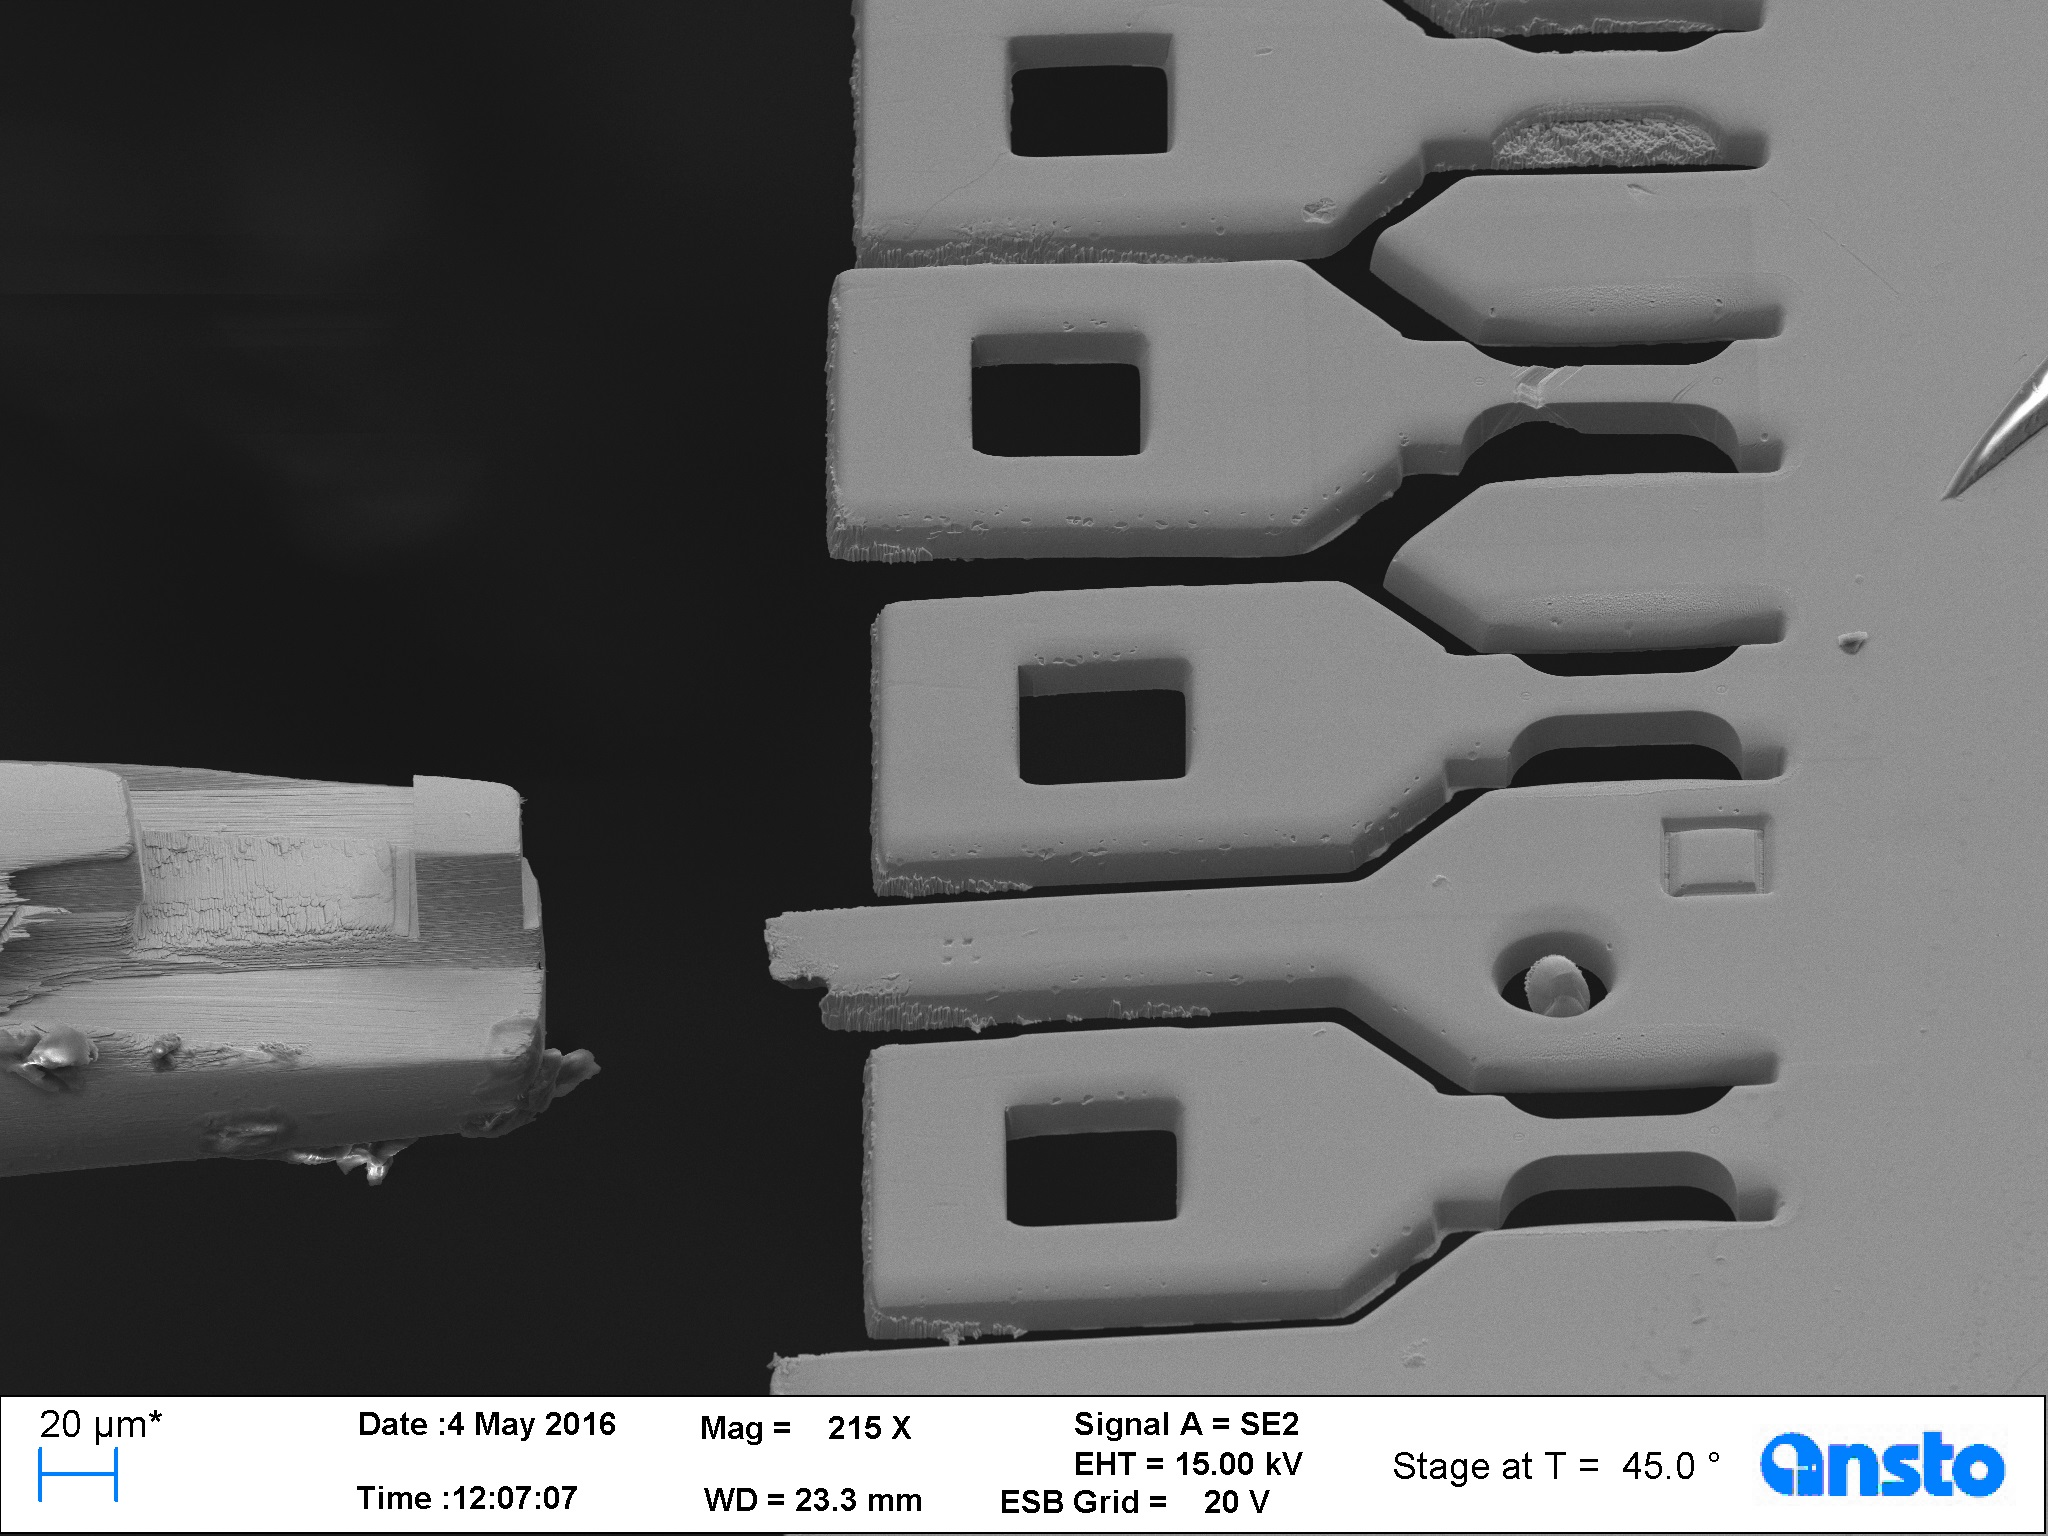
\includegraphics[width=\linewidth]{../data/Ni024.jpg}
        \caption[Stage for micropillar tensile tests.]{Stage for micropillar tensile tests. Ensemble setup, pillars are pulled from the square hole. They are allowed to freely move in the $yz$-plane.}
    \end{subfigure}
    ~
    \begin{subfigure}[t]{0.45\linewidth}
        \centering
        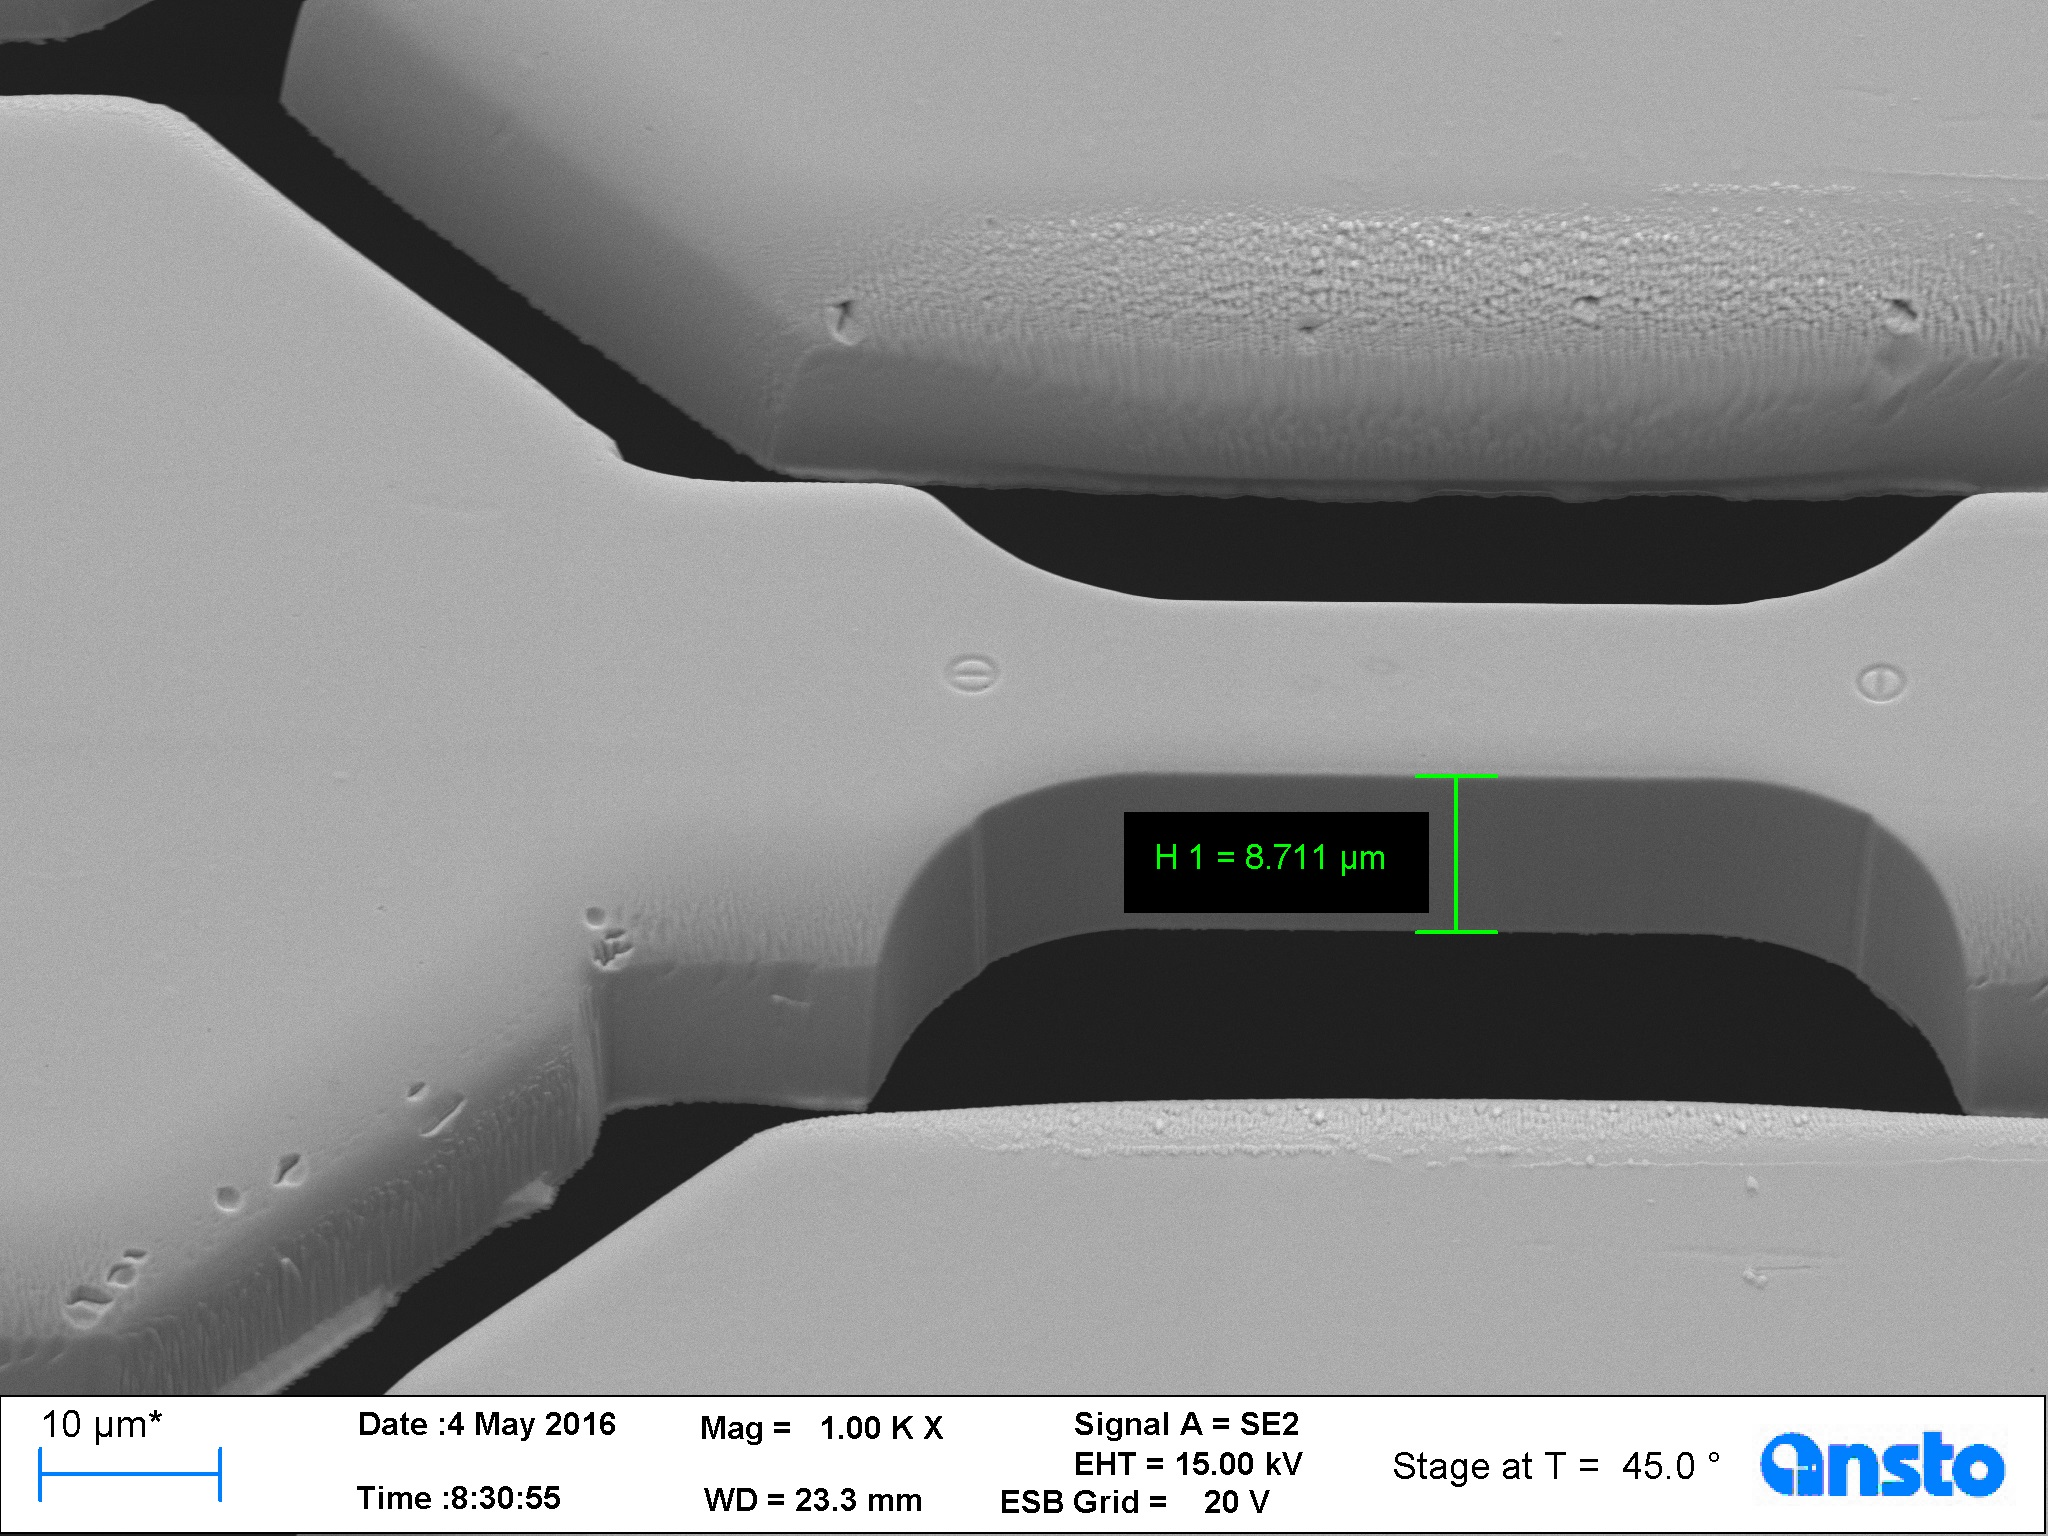
\includegraphics[width=\linewidth]{../data/Ni000.jpg}
        \caption[Close up of the initial state of a single pillar.]{Close up of the initial state of a single pillar. Camera is at $\SI{45}{\degree}$, square cross-section measures $\SI{12}{\micro\metre}$ per side, length is $\sim \SI{30}{\micro\metre}$.}
    \end{subfigure}
    \caption{Experimental stage for tensile tests on Ni micropillars.}
    \label{f:expSetup}
\end{figure}
The load was applied until the pillars failed by necking, as shown in \cref{f:tensileFailure}.
\begin{figure}
    \centering
    \begin{subfigure}[t]{0.3\linewidth}
        \centering
        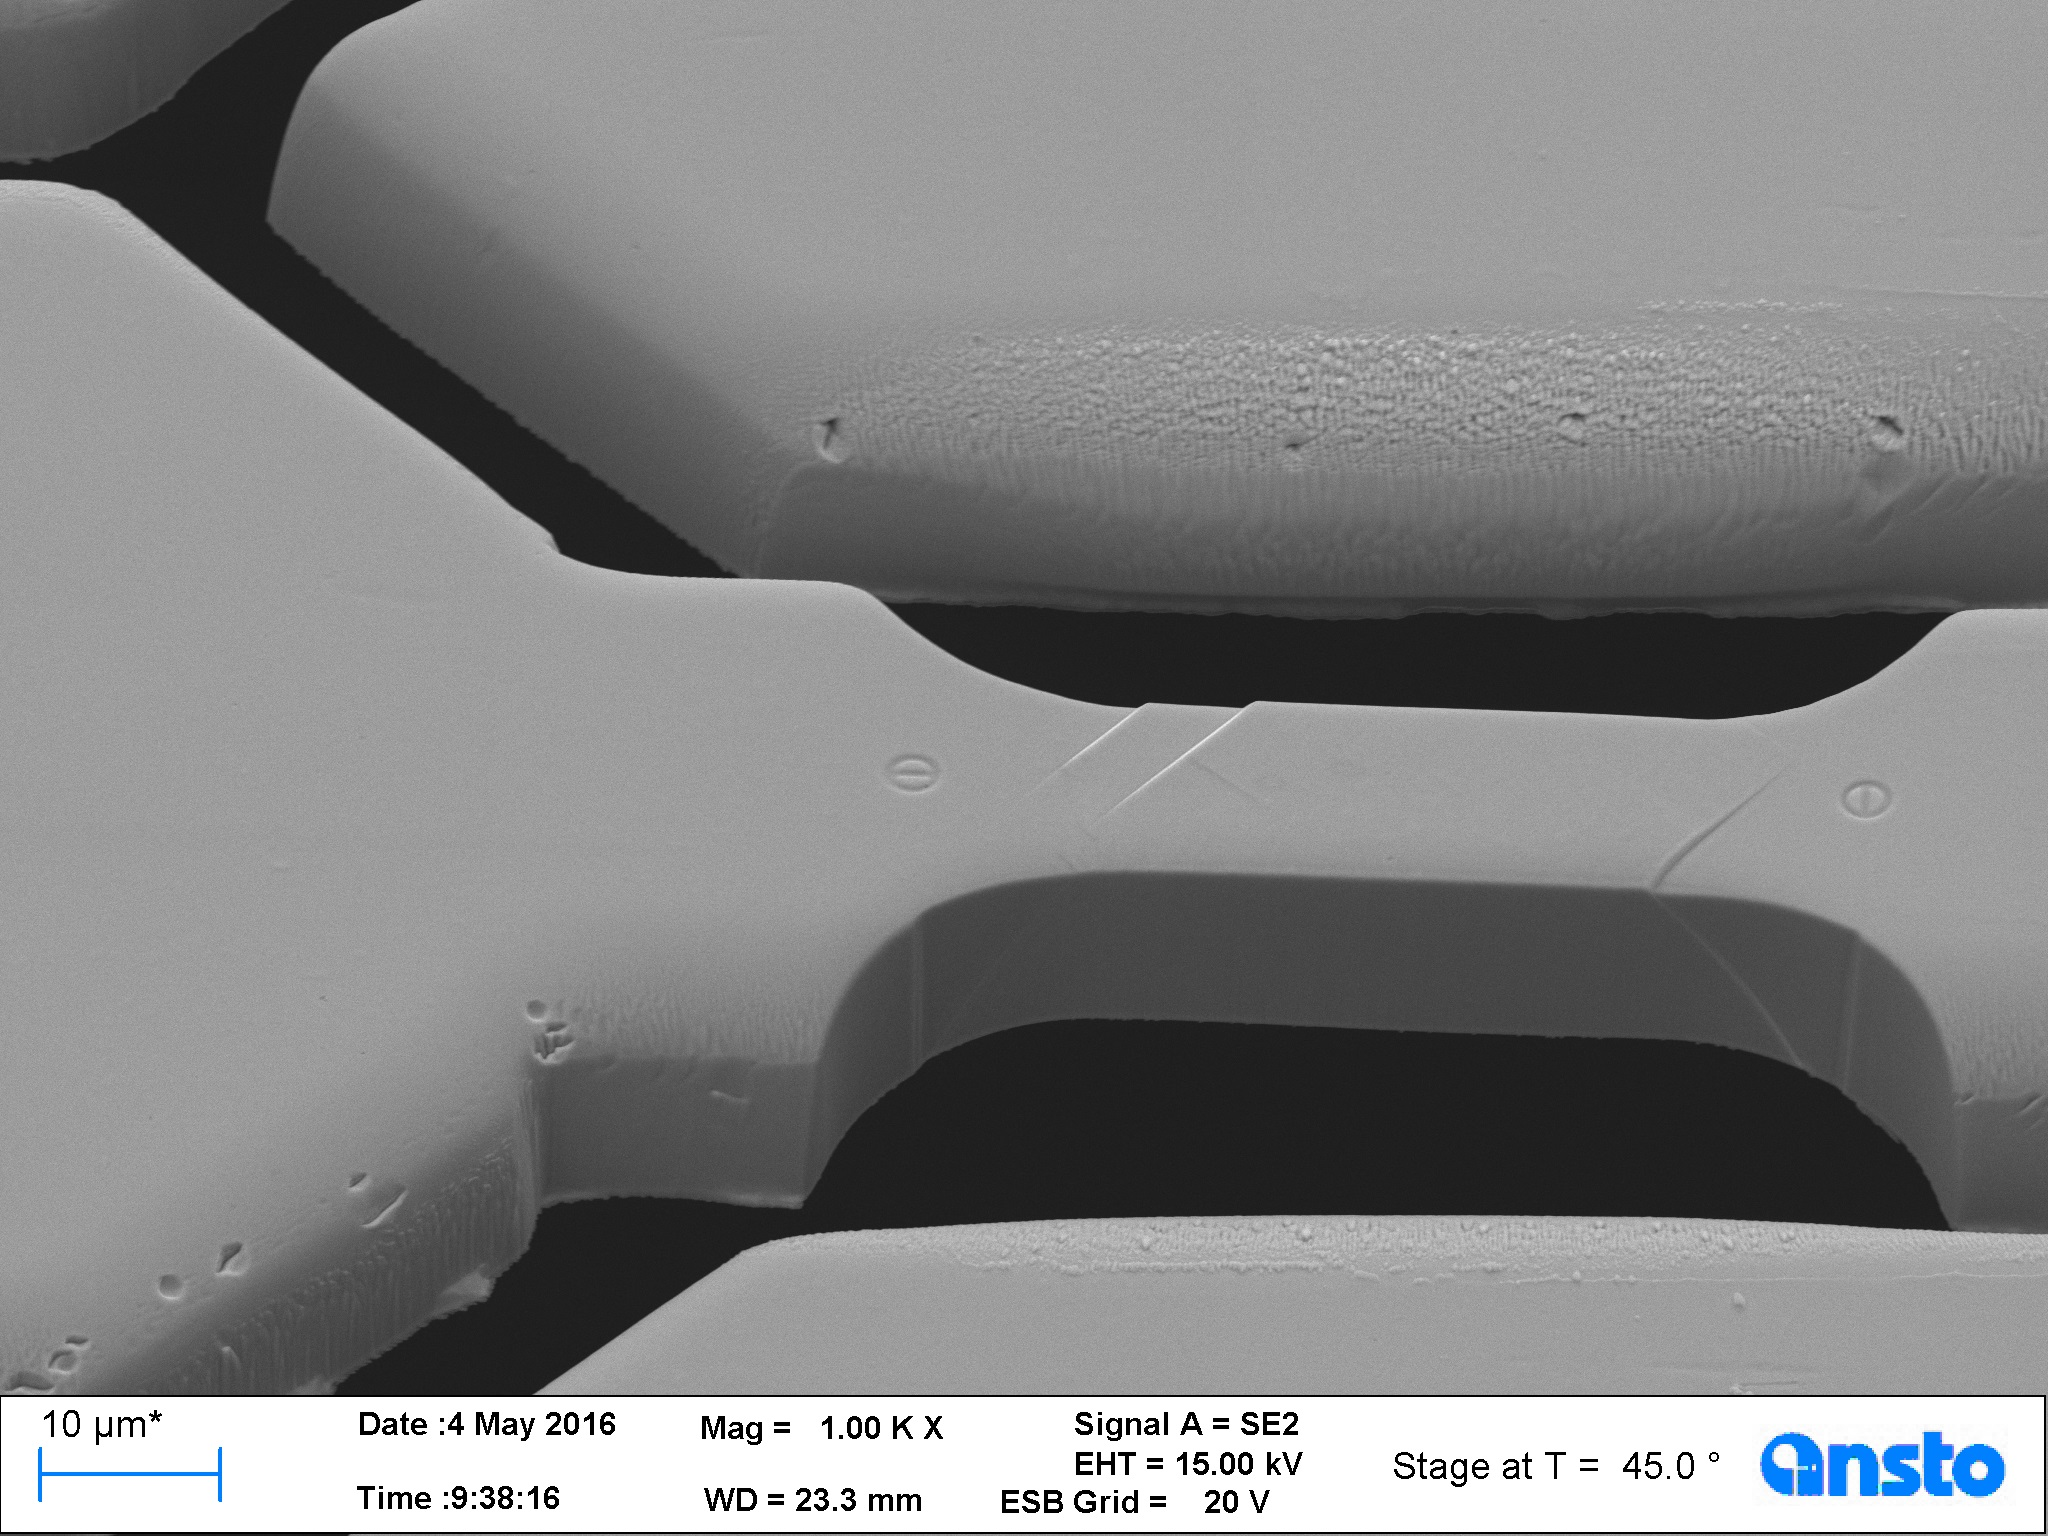
\includegraphics[width=\linewidth]{../data/Ni016.jpg}
    \end{subfigure}
    ~
    \begin{subfigure}[t]{0.3\linewidth}
        \centering
        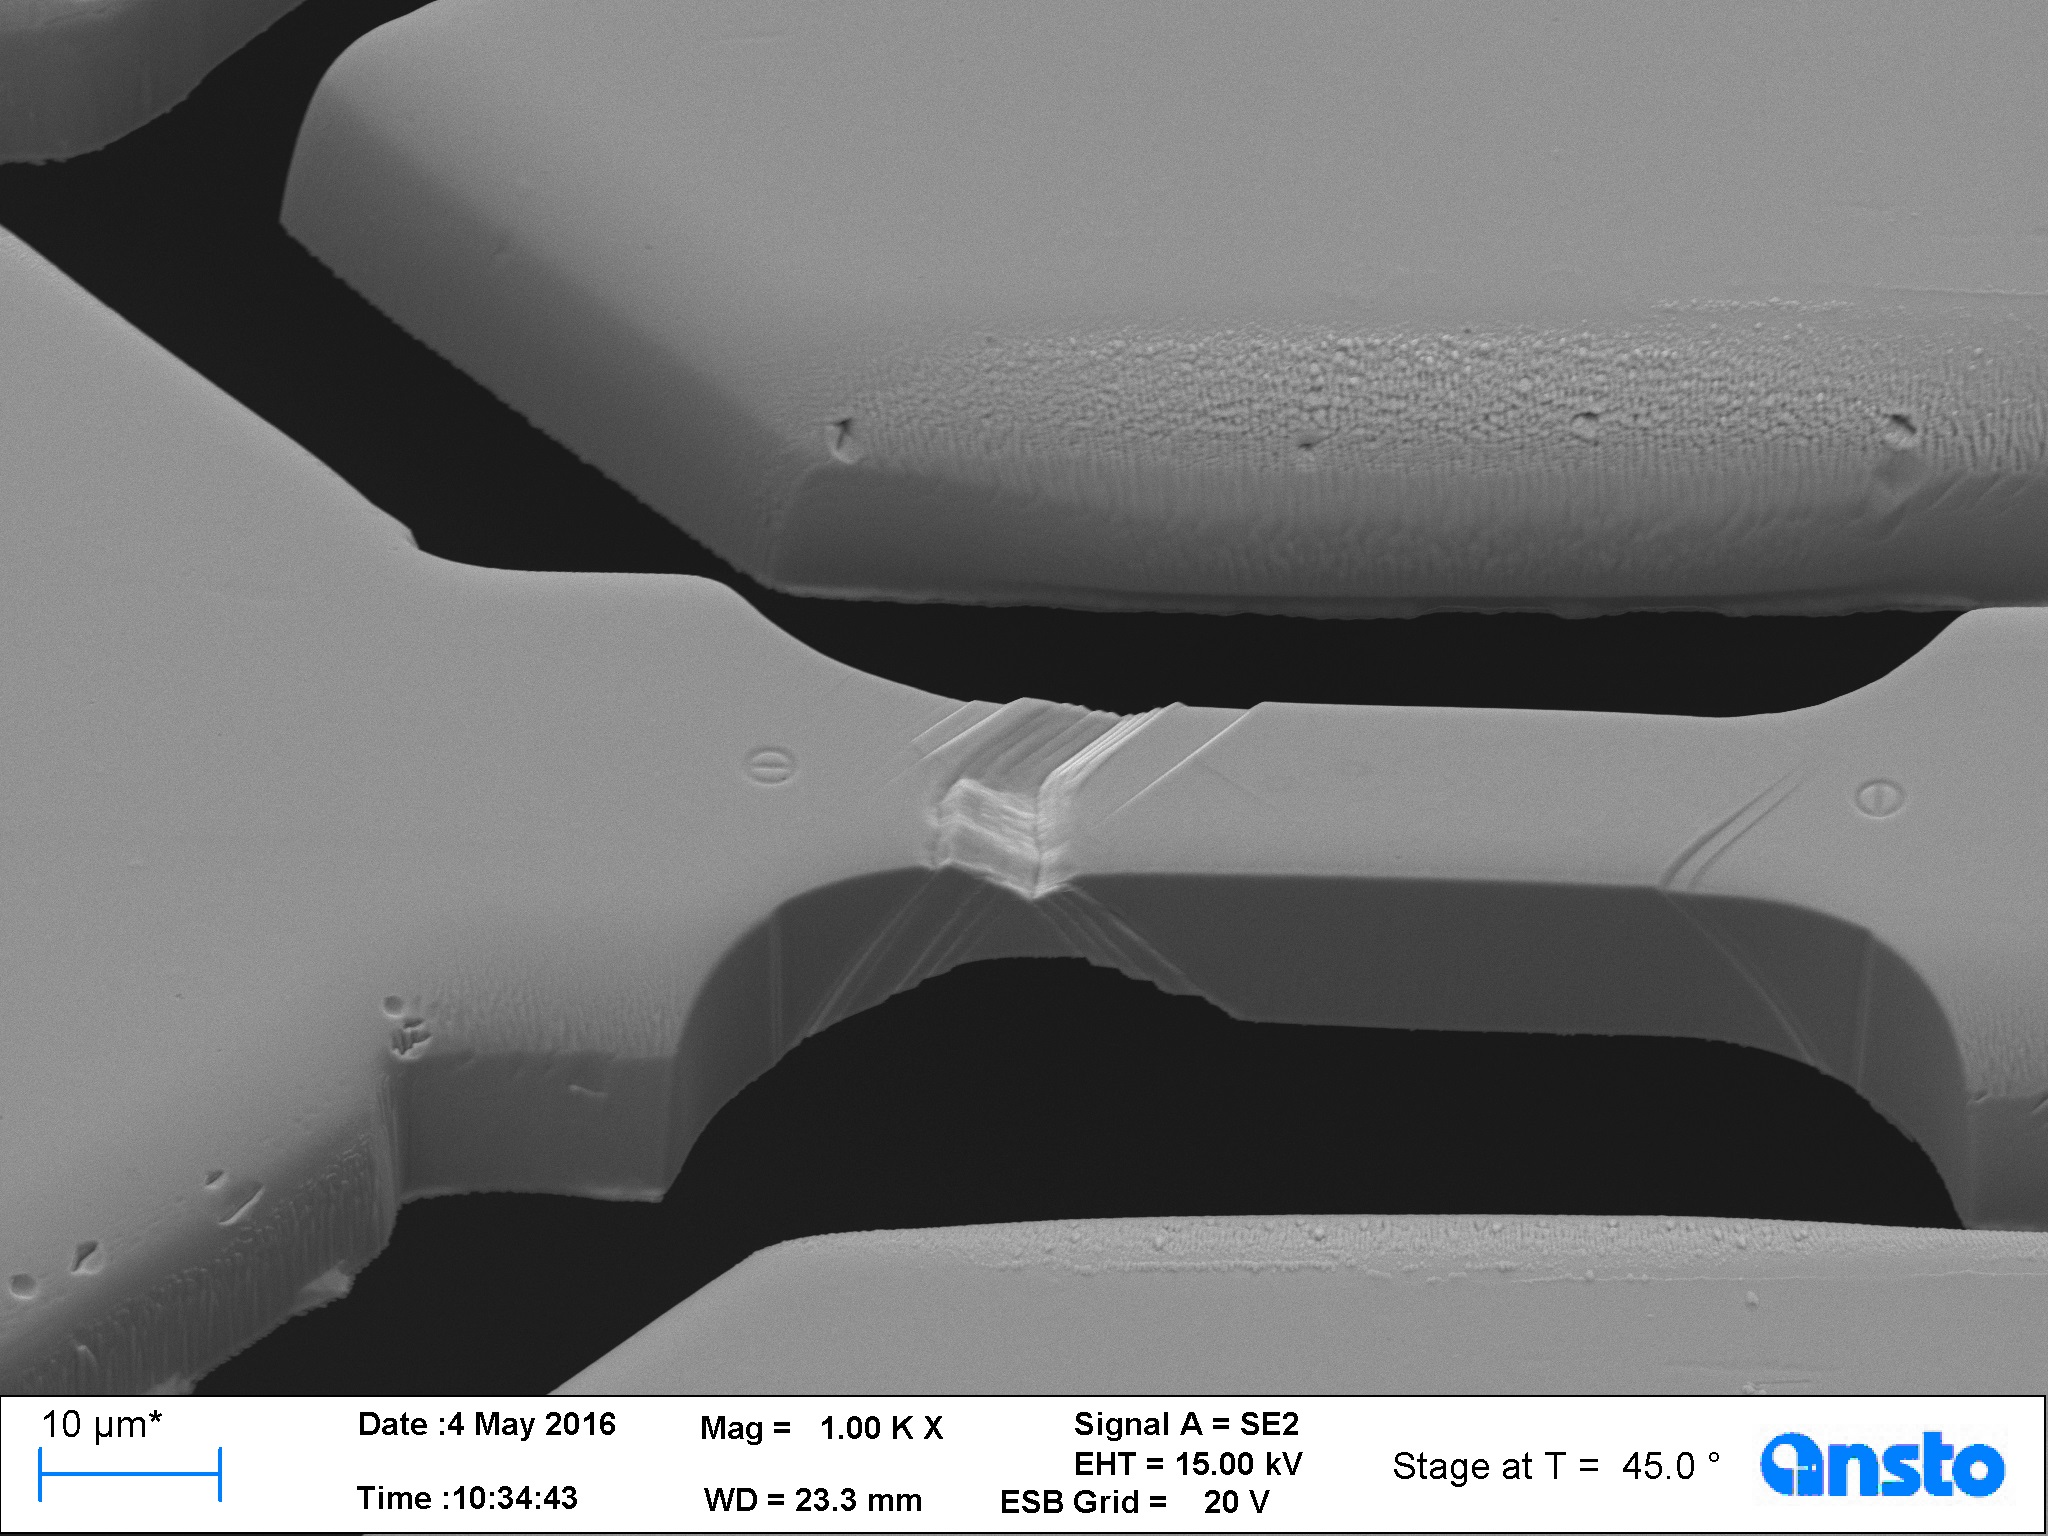
\includegraphics[width=\linewidth]{../data/Ni023.jpg}
    \end{subfigure}
    ~
    \begin{subfigure}[t]{0.3\linewidth}
        \centering
        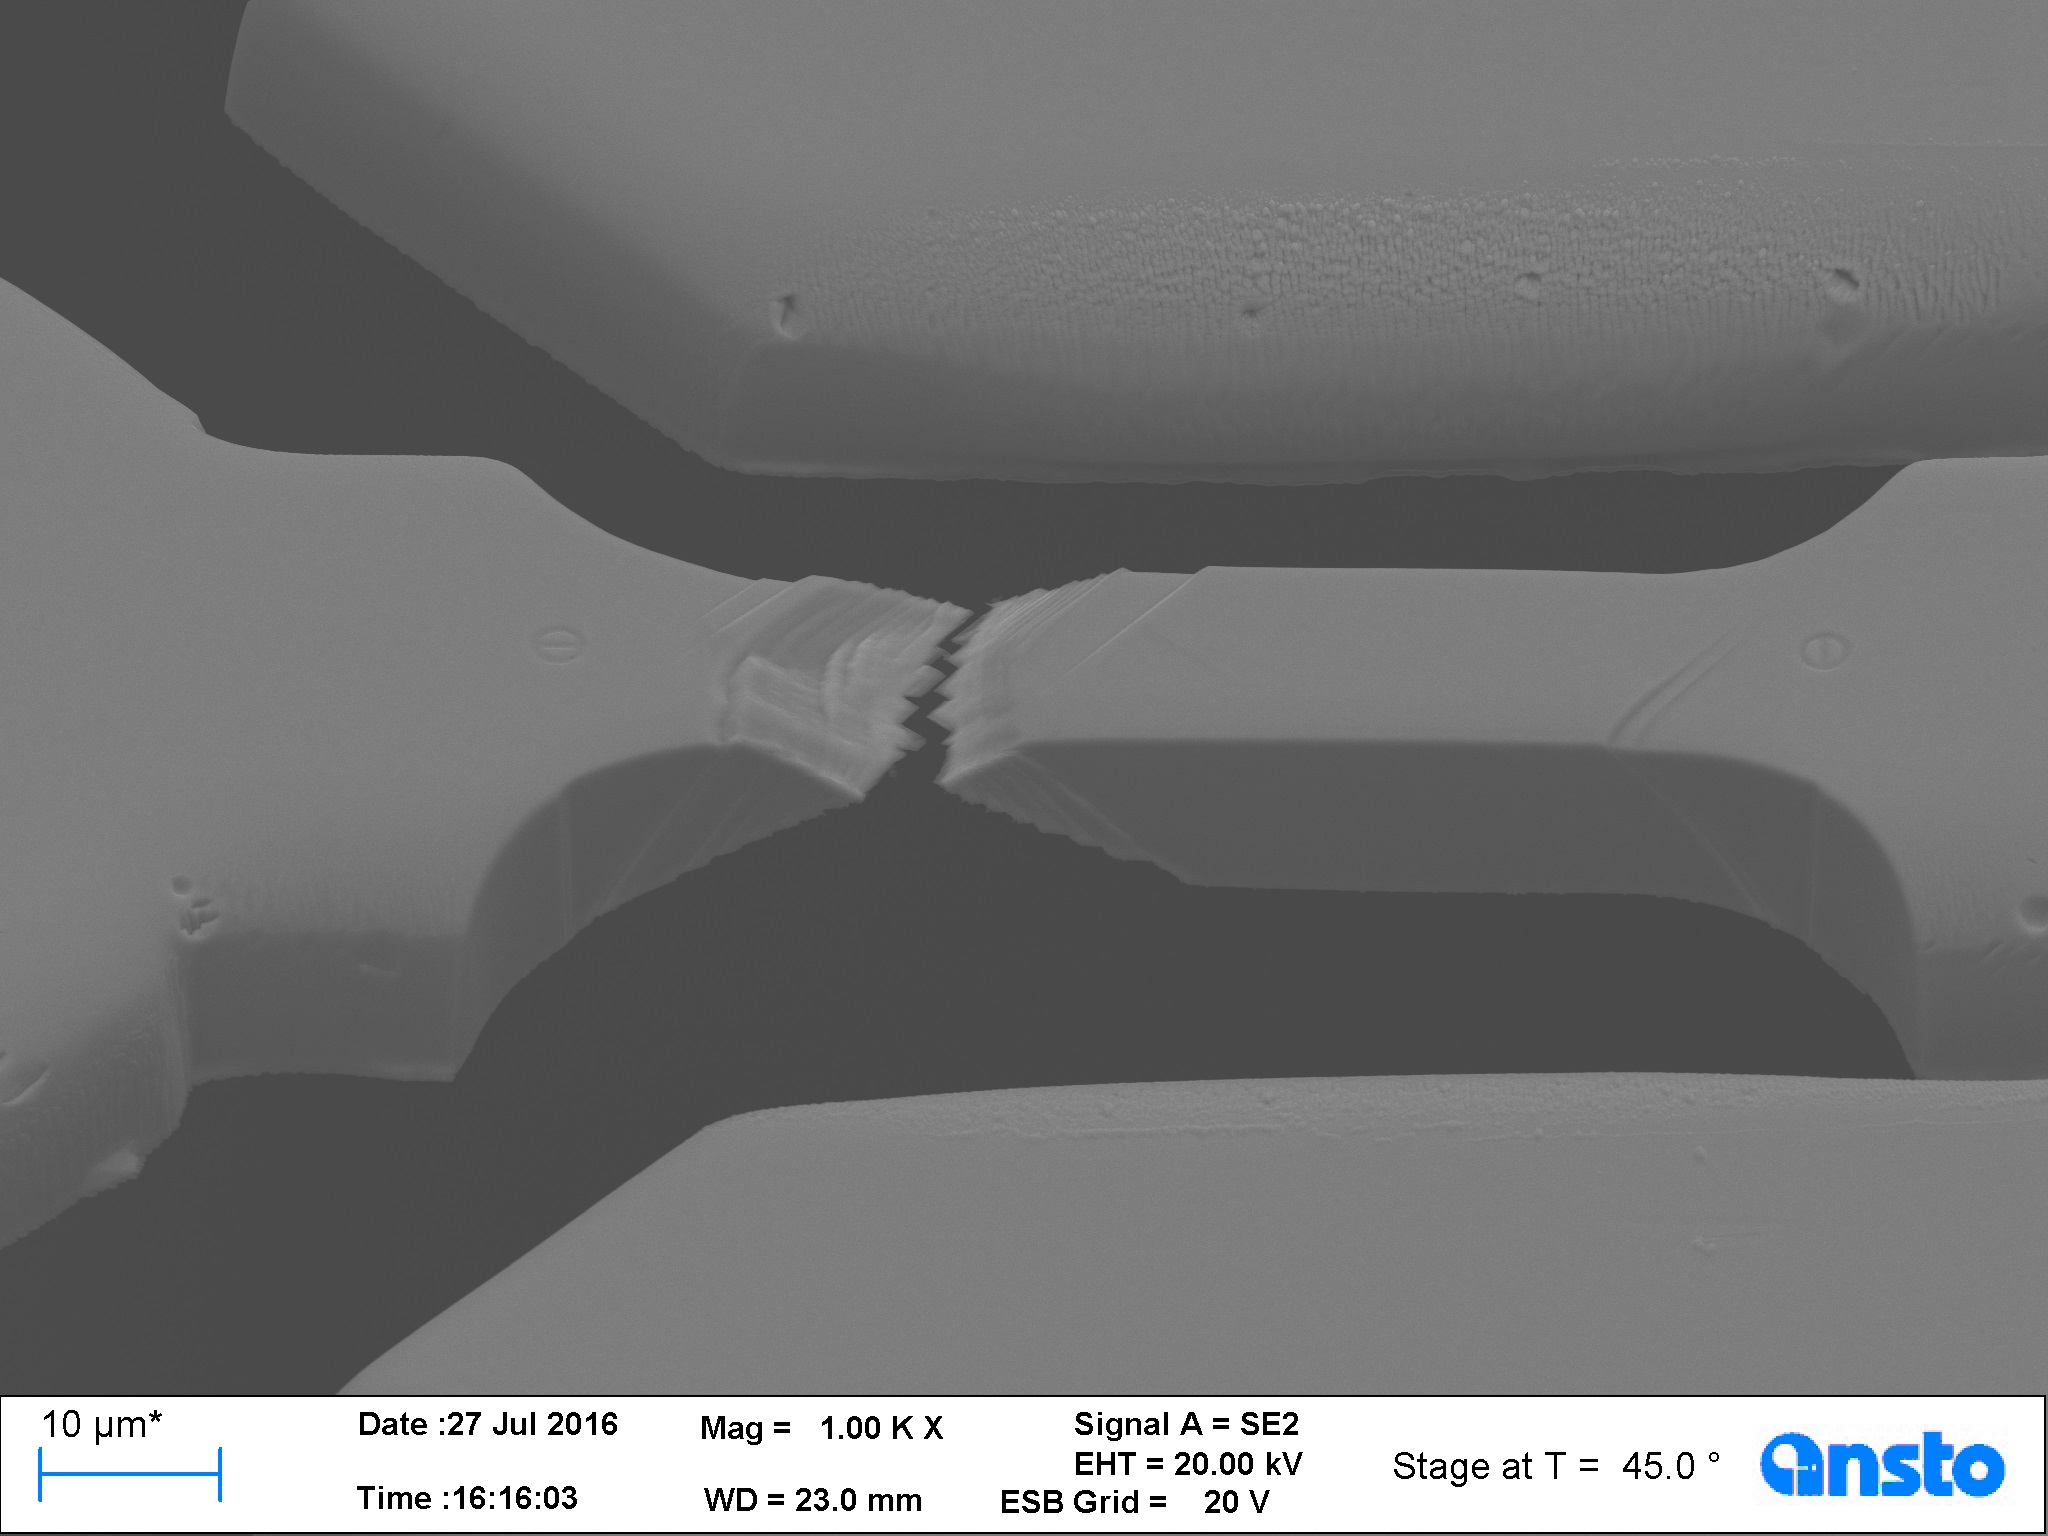
\includegraphics[width=\linewidth]{../data/Ni039.jpg}
    \end{subfigure}
    \caption{Tensile tests taken to failure.}
    \label{f:tensileFailure}
\end{figure}

It is worth noting that the timescale of dislocation plasticity simulations make them unsuitable to simulate the entirety of the experiments. EasyDD does not have a damage law, so it cannot account for fracture. Simulation loading rates are also necessarily higher than experimental ones as discrete dislocation dynamics time scales are on the order of \si{\nano\second}.

\subsection{Dislocation plasticity setup}
\label{ss:modelSetup}

The material parameters of the samples were also not known, so they were estimated from comercially available manufacturing spec sheets and measurements reported from literature. The exact values used for the lattice parameter, shear modulus and Poisson ratio are: $a \coloneqq \SI{3.499}{\angstrom}$, $ \mu  \coloneqq \SI{79}{\giga\pascal}$, $\nu \coloneqq 0.31$ respectively. The lattice parameter is from \cite{ni_lattice} and the othters are the mean of the upper and lower values reported by \cite{azom_nickel}.

We used prismatic loops with four sides as Frank-Reed sources to seed the domain with dislocations. Each side of the square sources had two segments of equal length. Because we used Fran-Reed sources, only two sides per source were allowed to move, the others were pinned.

Preliminary simulations showed the initially assumed dislocation density necessitated the initial sources be quite small, so the yield stress of the simulation was much greater than what was experimentally observed. We therefore dropped the number of sources to a single seed loop per active slip system, while increasing the size of each source. For the $\langle 1\, 0\, 0 \rangle$ loading direction, this was 8 loops, and for $\langle 1\, 1\, 0 \rangle$ it was only 4; \cref{t:slipSystems} contains the active slip systems for both scenarios.
\begin{table}
    \centering
    \caption{Active FCC slip systems for prismatic loops in the $\langle 1\, 0\, 0 \rangle$ and $\langle 1\, 1\, 0 \rangle$ tensile loading directions.}
    \label{t:slipSystems}
    \begin{tabular}{rcl}
        \toprule
        Loading direction                            & Slip plane    & Burgers vector           \\
        \midrule
        \multirow{8}{*}{$\langle 1\, 0\, 0 \rangle$} & $(1\, 1\, 1)$ & $[1\, \overline{1}\, 0]$ \\
                                                     & $(1\, 1\, 1)$ & $[1\, \overline{1}\, 0]$ \\
                                                     & $(1\, 1\, 1)$ & $[1\, \overline{1}\, 0]$ \\
                                                     & $(1\, 1\, 1)$ & $[1\, \overline{1}\, 0]$ \\
                                                     & $(1\, 1\, 1)$ & $[1\, \overline{1}\, 0]$ \\
                                                     & $(1\, 1\, 1)$ & $[1\, 0\, \overline{1}]$ \\
                                                     & $(1\, 1\, 1)$ & $[1\, 0\, \overline{1}]$ \\
                                                     & $(1\, 1\, 1)$ & $[1\, 0\, \overline{1}]$ \\
        \midrule
        \multirow{4}{*}{$\langle 1\, 1\, 0 \rangle$} & $(1\, 1\, 1)$ & $[1\, \overline{1}\, 0]$ \\
                                                     & $(1\, 1\, 1)$ & $[1\, \overline{1}\, 0]$ \\
                                                     & $(1\, 1\, 1)$ & $[1\, \overline{1}\, 0]$ \\
                                                     & $(1\, 1\, 1)$ & $[1\, 0\, \overline{1}]$ \\
        \bottomrule
    \end{tabular}
\end{table}
To minimise computation expenditure, we only included these active slip systems in our simulations. This obviously does not fully represent reality, but it saves simulations from having to resolve as many collisions and topological operations as would otherwise occur. Regardless of this decision, the simulations still managed to do an unexpectedly great job at quantitatively, and qualitatively reproducing the experimentally measured stress-strain curves as discussed in \cref{s:NiResults}.

The pillar length was defined as $\SI{36}{\micro\metre}$, or $3\times$ the length of one of the sides of the square cross-section. The extra length acts as a buffer zone for simulating dislocations moving into the bulk, where they pile up. In the simulation, they get pinned to the end of the cantilever, as per \cref{c:surfRem}. The initial FR sources were random-uniformly distributed within the central $80\%$ of the domain, i.e. $x \in [0.1X, 0.9X]$, where $x$ is a point along dimension $X$. Given the fact that the number of sources was quite low, various distributions were generated until we arrived at one that spanned the whole domain, rather than clustered about a region.

We define surface node sets $\left\{\forall (x, y, z) \in [0,\, 1] \vert S_{xyz} \in \partial \hat{V}\right\}$, where $\hat{V}$ is a unit volume such that $S_{000}$ denotes the node at the origin, $S_{x00}$ the $x$-axis spanning edge at $y,\, z=0$, and $S_{xy0}$ the $xy$-plane at $z=0$. We use these node sets to define our Neuman (displacement) boundary conditions as follows,
\begin{subequations}
    \begin{align}
        u_x(0, y, z) & = 0    \\
        u_y(0, Y, z) & = 0    \\
        u_z(0, y, 0) & = 0    \\
        u_x(X, y, z) & = U\,. \\
        % S_{0yz},\, S_{0y0},\, S_{0y1},\, S_{00z},\, S_{01z},\, S_{000},\, S_{001},\, S_{010},\, S_{011} & \gets u_x = 0        \\
        % S_{01z},\, S_{010},\, S_{011}                                                                   & \gets u_y = 0        \\
        % S_{0y0},\, S_{010},\, S_{000}                                                                   & \gets u_z = 0        \\
        % S_{1yz},\, S_{1y0},\, S_{1y1},\, S_{10z},\, S_{11z},\, S_{100},\, S_{101},\, S_{110},\, S_{111} & \gets u_x = U > 0\,.
    \end{align}
\end{subequations}
Where $X$, $Y$, $Z$ are the limits of the FE domain. Once mapped to our simulated cuboid geometry, it looks like \cref{f:tensileSetup}. All other degrees of freedom are free to move.
\begin{figure}
    \centering
    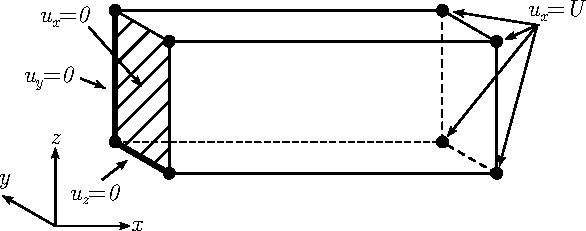
\includegraphics[width=0.8\linewidth]{tensileSetup.pdf}
    \caption[Displacement boundary conditions for dislocation plasticity modelling of single crystal, micro-tensile tests.]{Displacement boundary conditions for dislocation plasticity modelling of single crystal, micro-tensile tests.}
    \label{f:tensileSetup}
\end{figure}

In EasyDD, time is defined in units of shear modulus \cref{eq:timeConversion},
\begin{align}\label{eq:timeConversion}
    t_{\rvar{real}} & = t_{\rvar{sim}} \dfrac{B}{\mu}\,.
\end{align}
In EasyDD the dislocation mobility, $B \coloneqq 1$ and $\mu \coloneqq 1$. However, $B$ has units of $\si{\pascal\,\second\,b^{-1}}$, and $\mu$ units of $\si{\pascal}$. In order to estimate our loading rate, we used a generic value for an FCC transition metal of $B = \SI{1e-4}{\pascal\,\second}$, and used similar heuristics as described in \cite[p.~237]{ddlab}.

The experimental loading rates were $\SI{5}{\nano\metre\per\second}$ and $\SI{500}{\nano\metre\per\second}$, give simulation loading rates that are far too low for the timescales we can simulate. However, as mentioned in \cref{ss:matrix}, it is important that a quasistatic condition is met for the mobility functions to hold. We therefore chose a loading rate that enabled simulations to advance sufficiently, without overloading the system. We settled on multiplying the converted value\footnote{The converted value used in the simulations is $\left(\SI{5e-3}{\micro\metre}/a\right) \times \left(B /  \mu \right)$, where $a$ is the lattice parameter in micrometers, $B$ the dislocation mobility and $ \mu $ the magnitude of the shear modulus from \cref{eq:timeConversion}.} of the $\SI{5}{\nano\metre\per\second}$ loading rate by a factor of $5 \times 10^6$, which corresponds to a loading rate of $\SI{2.5}{\centi\metre\per\second}$. Any higher and the yield point increased, any lower and the simulations took much longer to advance without a significant change in the dislocation structure and stress-strain curve.

Furthermore, two source segment lengths were trialed. For the $\langle 1\, 0\, 0 \rangle$ loading direction we assumed two values for $\sigma_\rvar{y} = 183 \text{ and } \SI{142}{\mega\pascal}$, giving corresponding source perimeters of $3.4176 \text{ and } \SI{4.4047}{\micro\metre}$. For the $\langle 1\, 1\, 0 \rangle$ direction, we also used two values of $\sigma_\rvar{y} = 158 \text{ and } \SI{101}{\mega\pascal}$, corresponding to source perimeters of $ 3.4179 \text{ and } \SI{3.9587}{\micro\metre}$. The assumptions came from experimental values suggested by Alan and Dhriti, but had to be adjusted to account for the simulation's higher loading rate. We also did not directly use \cref{eq:yieldStress}, but $l = 2 \mu b / \sigma_\rvar{y}$, to account for the sources being at an angle with respect to the loading direction\footnote{Perhaps it would be more accurate to drop the factor of two and use the critically resolved shear stress instead of the yield stress directly, $\tau = \cos(\phi)\cos(\lambda) \sigma_\rvar{y}$, where $\phi$ and $\lambda$ are the angles between the applied stress, glide plane normal, and glide direction respectively. However, a number of much stronger assumptions and adjustments had already been made, and this worked satisfactorily.}. Thiis gave two source size parameters for each direction.

All simulations ran for approximately 5 weeks. They did not use the new power dissipation strategy for collision-separation because that development came a few weeks after the simulations started running, and other computational resources were of critical importance to other users.

\section{Results and discussion}
\label{s:NiResults}

The experimental measurements go up to fracture, well beyond the domain of dislocation plasticity simulations; they also discard the elastic region, and the early onset of plasticity as shown in \cref{sf:Ni100,sf:Ni110}. Conversely, dislocation plasticity simulations are limited to small strains, i.e. the part of the curves that typically fall below the experimental limit of detection as shown in \cref{sf:Ni100_DDD,sf:Ni110_DDD}. However, they can elucidate dislocation mechanisms behind plasticity. Here, dislocation plasticity serves as a bridge between the elastic and plastic regimes and lets us explore the mechanisms behind the differences in stress-strain curves between the $\langle 1\,0\,0 \rangle$ and $\langle 1\,1\,0 \rangle$ loading directions.
\begin{figure}
    \centering
    \begin{subfigure}[t]{0.45\linewidth}
        \centering
        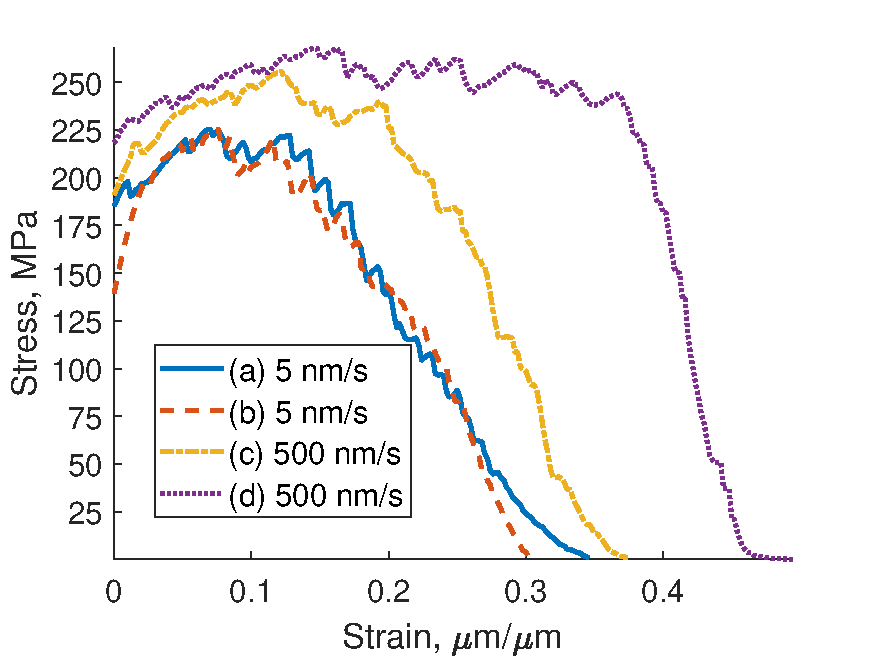
\includegraphics[width=\linewidth]{../data/Ni100.pdf}
        \caption{Experimental results of tensile loading of Ni in $\langle 1\, 0\, 0 \rangle$.}
        \label{sf:Ni100}
    \end{subfigure}
    ~
    \begin{subfigure}[t]{0.45\linewidth}
        \centering
        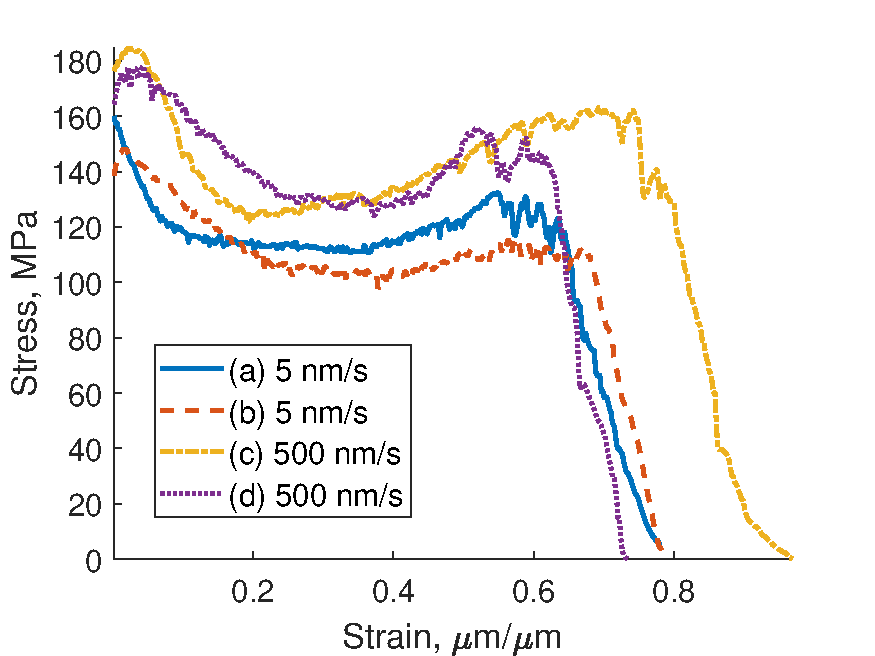
\includegraphics[width=\linewidth]{../data/Ni110.pdf}
        \caption{Experimental results of tensile loading of Ni in  $\langle 1\, 1\, 0 \rangle$.}
        \label{sf:Ni110}
    \end{subfigure}

    \begin{subfigure}[t]{0.45\linewidth}
        \centering
        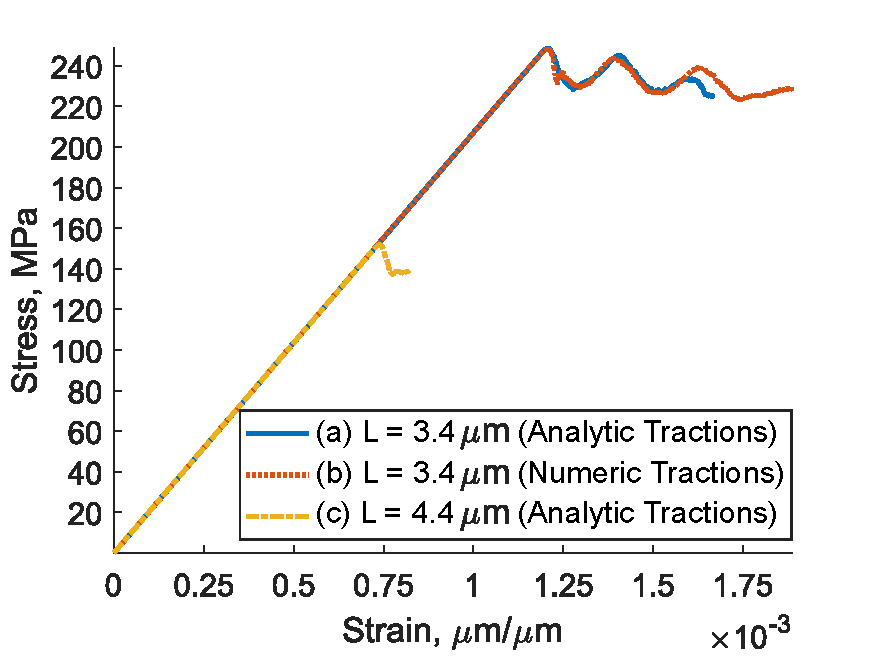
\includegraphics[width=\linewidth]{../data/Ni100_DDD.pdf}
        \caption[Dislocation-Plasticity simulation of tensile loading of Ni in $\langle 1\, 0\, 0 \rangle$.]{Dislocation-Plasticity simulation of tensile loading of Ni in $\langle 1\, 0\, 0 \rangle$. (a) and (b) use the same distribution of small sources, (c) uses a different distribution of larger ones. (a) uses analytic tractions and (b) numeric ones.}
        \label{sf:Ni100_DDD}
    \end{subfigure}
    ~
    \begin{subfigure}[t]{0.45\linewidth}
        \centering
        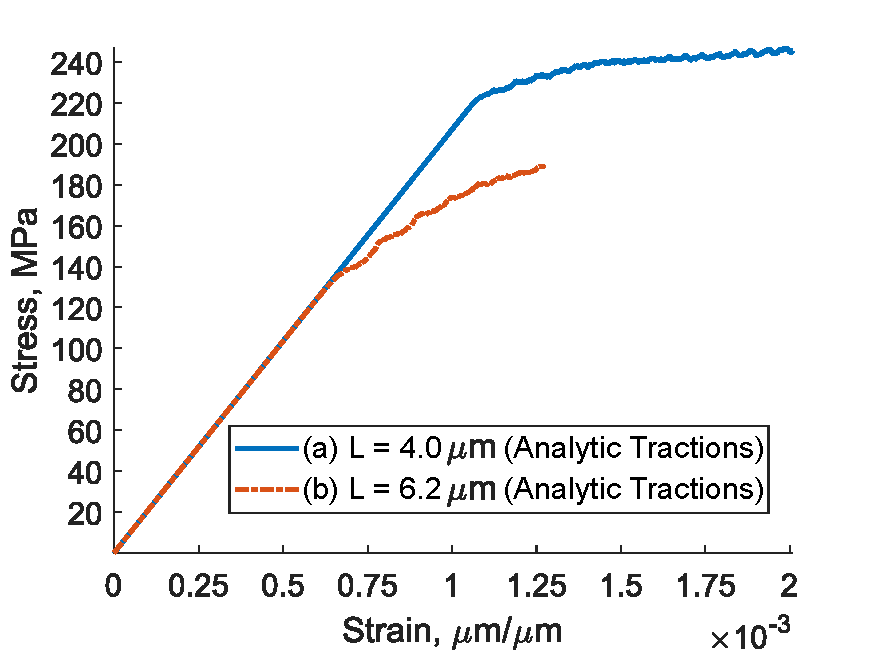
\includegraphics[width=\linewidth]{../data/Ni110_DDD.pdf}
        \caption[Dislocation-Plasticity simulation of tensile loading of Ni in $\langle 1\, 1\, 0 \rangle$.]{Dislocation-Plasticity simulation of tensile loading of Ni  in $\langle 1\, 1\, 0 \rangle$. (a) uses small sources, (b) uses a different distribution of larger ones.}
        \label{sf:Ni110_DDD}
    \end{subfigure}
    \caption{Experimental and simulated stress-strain curves of Ni micropillar tensile tests.}
    \label{f:NiStrainStress}
\end{figure}

\Cref{sf:Ni100,sf:Ni110} show the experimental strain stress curves for the $\langle 1\,0\,0 \rangle$ and $\langle 1\,1\,0 \rangle$, respecively. As expected, higher loading rates mean higher stresses overall, and different loading directions produce very different graphs. However, there is quite a large variation between samples even within similar loading rates. This points at dislocations having quite a large effect on the outcome of the experiment. The difference in shape between graphs of both loading directions also point to different slip systems activating at different points and behaving quite differently from each other.

Looking at the low displacement rate curves, (a) and (b) in \cref{sf:Ni100}, it is evident both are quite similar for most of their domain. However, one of the samples yields close to $\SI{140}{\mega\pascal}$ and fails at $30\%$ strain, while the other yields at around $\SI{180}{\mega\pascal}$ and fails closer to $35\%$. These are not insignificant differences, especially at small scales. However, the bulk of the curves look quite similar to one another, and very different to the higher loading rate curves.

Conversely, the high loading rate curves in, (c) and (d) in \cref{sf:Ni100}, are very different to one another. Curve (c) yields at approximately the same point as (a), and the difference in its failure strain and that of curve (a) is less than the difference between curves (a) and (b). That said, curves (c) and (d) are subjected to higher stresses and fail at higher strains than (a) and (b).

Unfortunately, dislocation plasticity simulations cannot probe such high strains and low loading rates, but it would be interesting to investigate the dislocation mechanisms behind this increased plasticity. One has to wonder whether this is a result of kinetic processes that are typically ignored in dislocation dynamics. However, it may also be the fact that the number of samples is quite limited, so the differences may be due to heterogeneity between samples.

Sadly, sophisticated statistical analyses cannot be performed due to the low number of samples, but we can at least perform a principal component analysis (PCA) and plot the dominant components, as shown in \cref{sf:Ni100_pca}, to see whether the differences between low and high loading rates---respectively denoted by blue triangles (\textcolor{matlabBlue}{$\blacktriangle$}) and orange circles (\textcolor{matlabOrange}{$\bullet$})---are significant. With so few data points, a clustering analysis would not yield quality information.
\begin{figure}
    \centering
    \begin{subfigure}[t]{0.45\linewidth}
        \centering
        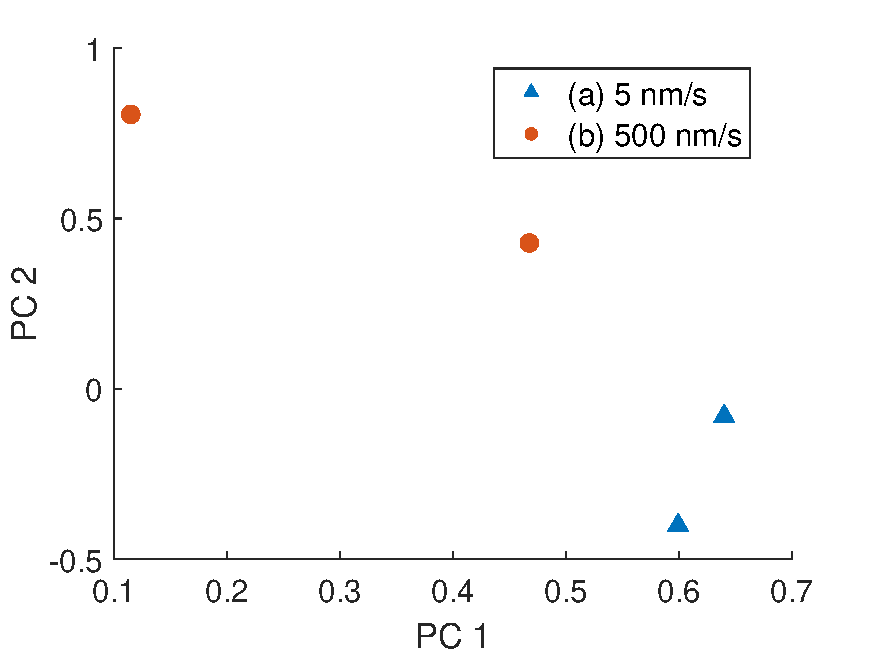
\includegraphics[width=\linewidth]{../data/Ni100_pca.pdf}
        \caption[First two principal components of the Ni stress-strain curves in $\langle 1\,0\,0 \rangle$.]{First two principal components of the Ni stress-strain curves in $\langle 1\,0\,0 \rangle$. First and second principal components respecitvely correspond to $79.41\%$ and $19.05\%$ of the observed variance between curves.}
        \label{sf:Ni100_pca}
    \end{subfigure}
    ~
    \begin{subfigure}[t]{0.45\linewidth}
        \centering
        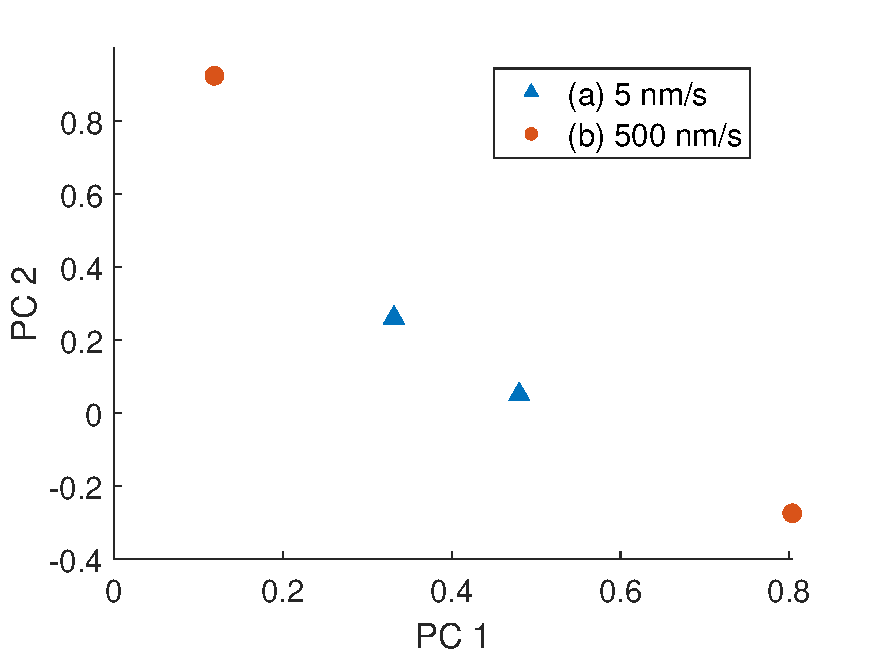
\includegraphics[width=\linewidth]{../data/Ni110_pca.pdf}
        \caption[First two principal components of the Ni stress-strain curves in $\langle 1\,1\,0 \rangle$.]{First two principal components of the Ni stress-strain curves in $\langle 1\,1\,0 \rangle$. First and second principal components respecitvely correspond to $70.61\%$ and $26.21\%$ of the observed variance between curves.}
        \label{sf:Ni110_pca}
    \end{subfigure}
    \caption{Blue triangles (\textcolor{matlabBlue}{$\blacktriangle$}) correspond to the $\SI{5}{\nano\metre\per\second}$ loading rate, orange circles (\textcolor{matlabOrange}{$\bullet$}) that of $\SI{500}{\nano\metre\per\second}$.}
    \label{f:Ni_pca}
\end{figure}

As expected, the low loading rate measurements cluster together, hinting at similar behaviour. Moreover, the higher loading rates have a larger spread. The Eucledian distance from one of them is even smaller to both low loading rate measurements, than it is to its high loading rate counterpart. More measurements are needed to draw conclusions as to why this is the case. Regardless, it is relatively safe to assume the loading rate has a noticeable effect when loading the $\langle 1\, 0\, 0 \rangle$ direction for these specific rates. Such information is relevant for our simulations, as their loading rates were much higher than these, so we must expect those curves to behave accordingly, and our conclusions must be extrapolated with this in mind.

The story is much different for the $\langle 1\, 1\, 0 \rangle$ loading direction. All graphs in \cref{sf:Ni110} look quite similar. They are markedly different to those in \cref{sf:Ni100}, but among themselves there do not seem to be large differences between low loading rate curves, (a) and (b), and high loading rate ones, (c) and (d). Having said that, curves (c) and (d) consistently experience higher stresses than (a) and (b). With so few samples, it is hard to say whether there is a notable difference.

\Cref{sf:Ni110_pca} confirms this, the Eucledian distance between both low loading rate curves (\textcolor{matlabBlue}{$\blacktriangle$}) is much smaller to one another than that between both high loading rate curves (\textcolor{matlabOrange}{$\bullet$}). With only two data points for each measurement, it is very difficult to assert whether there is a relationship between the first and second principal components that can be used to correlate a curve to its loading rate. We therefore cannot draw satisfacotry conclusions whether such differences in loading rate have much of an effect. Conventional wisdom is that it will, but we cannot quantify how much, so we must tread with care.

Given the computational expense of simulations we cannot perform a meaningful PCA and compare the results to the experimental measurements as we do not have enough samples, and their maximal strains are well below the experimentally measured ones.

Qualitatively and quantitatively, the simulations do a surprisingly good job at reproducing the experimental stress-strain curves. Comparing the yield points and features of \cref{sf:Ni100,sf:Ni110} tith those of \cref{sf:Ni100_DDD,sf:Ni110_DDD} shows remarkable agreement between them. While the simulations cannot reach the same strains as the experiments, they appear to fall within experimental variation, excepting curve (a) of \cref{sf:Ni110_DDD}.

That said, we must be aware that the loading rate is 5 million times higher than $\SI{5}{\nano\meter\per\second}$. As previously mentioned, this loading rate was arrived at by finding the highest loading rate that would not exponentially increase the yield point. However, this does not mean lower loading rates do not decrease the yield point, they do, just not very drastically. They are also impractically slow for our needs.

It is also interesting to note that this was achieved with a very small number of initial sources, only one per active slip system, contrary to the originally assumed 10 dislocations \si{\micro\metre^{-2}}. They were also all prismatic, uniform in both size and shape. These are not wholly unreasonable assumptions, but they are definitely not strictly true, yet they did a remarkable job.

The appeal of dislocation plasticity is correlating dislocation dynamics to plastic behaviour. In general, stresses are relaxed as the total internal dislocation length increases.

The ``bumpy'' quality of the stress-strain curves in $\langle 1\, 0\, 0 \rangle$, as shown in \cref{sf:Ni100,sf:Ni100_DDD}, is the result of how quickly the internal dislocations grow. \Cref{f:Ni100_bumps} shows the dislocation structures and corresponding stress-strain curve for simulation (a) in \cref{sf:Ni100_DDD}. It can be observed that the slope of the peaks and valleys of the ``bumps'' correspond to how quickly the total internal dislocation length is growing. Upward slopes correspond to rapidly decreasing internal dislocation length. Conversely, downward slopes correspond rapidly increasing internal dislocation length. Of course, exited dislocations contribute to the relaxation of stresses via the creation of slip steps, but once they have left the simulation domain, their contributions remain static.
\begin{figure}
    \centering
    \begin{subfigure}[t]{\linewidth}
        \centering
        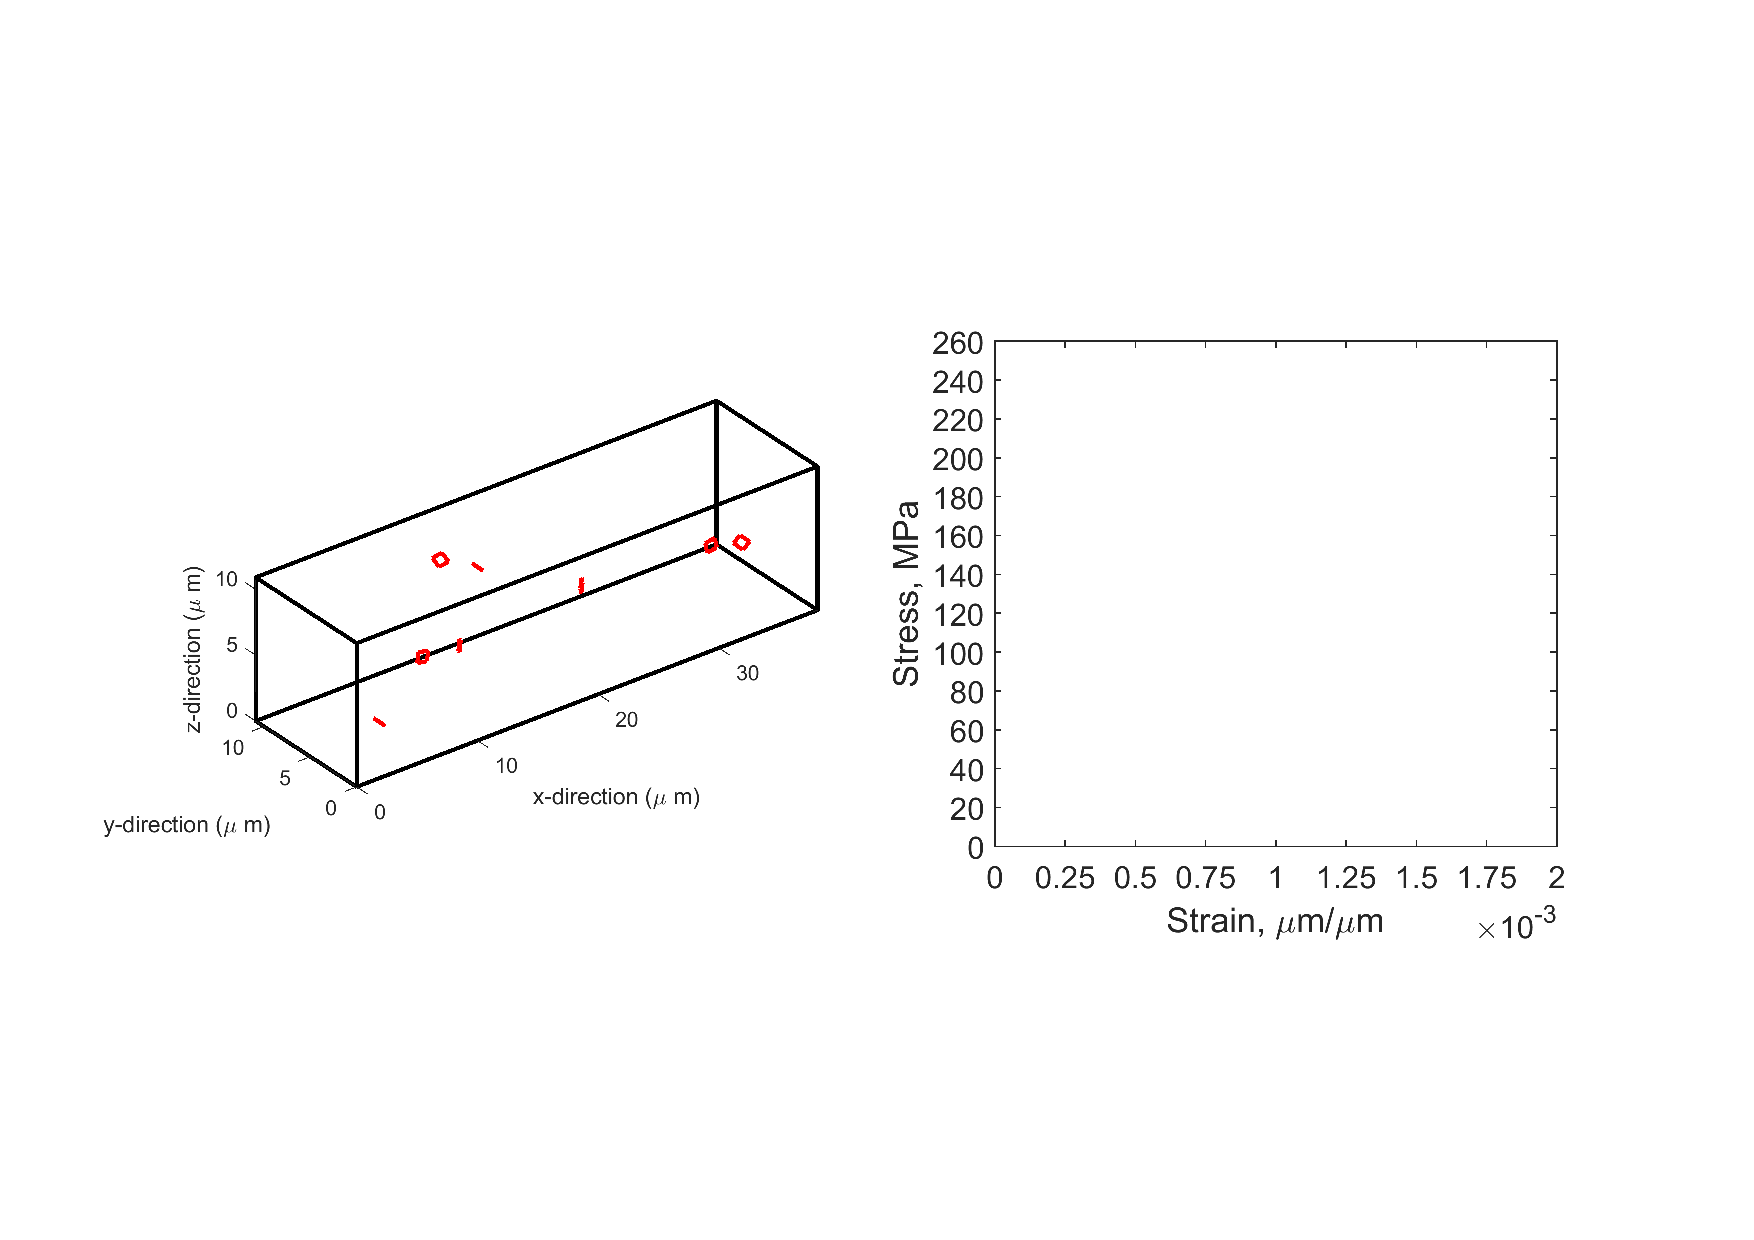
\includegraphics[trim={1.75cm 5cm 2.5cm 5.5cm},clip,width=\linewidth]{../data/11-Mar-2021_8_tensile_ni_100_0.pdf}
        \caption{Initial structure.}
    \end{subfigure}

    \begin{subfigure}[t]{\linewidth}
        \centering
        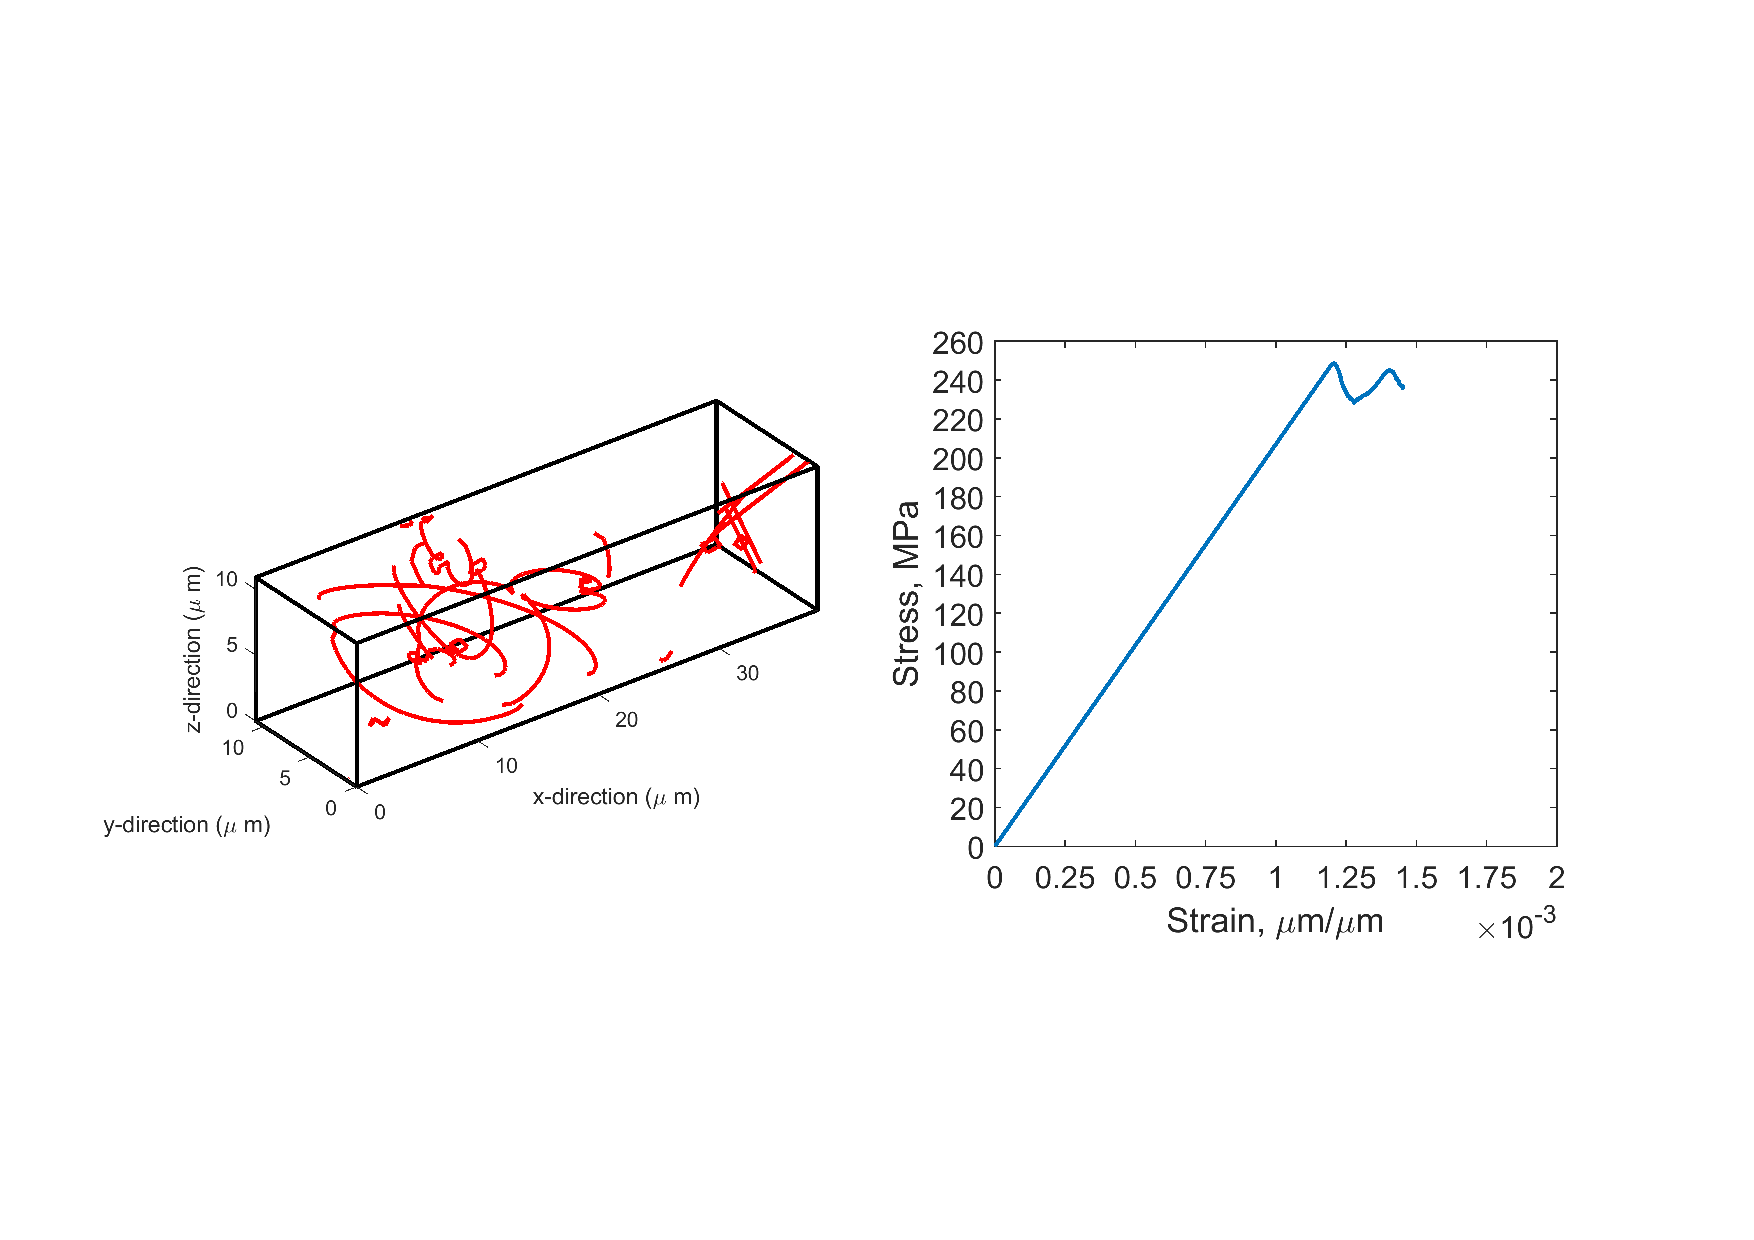
\includegraphics[trim={1.75cm 5cm 2.5cm 5.5cm},clip,width=\linewidth]{../data/11-Mar-2021_8_tensile_ni_100_60000.pdf}
        \caption{Downward slope.}
    \end{subfigure}

    \begin{subfigure}[t]{\linewidth}
        \centering
        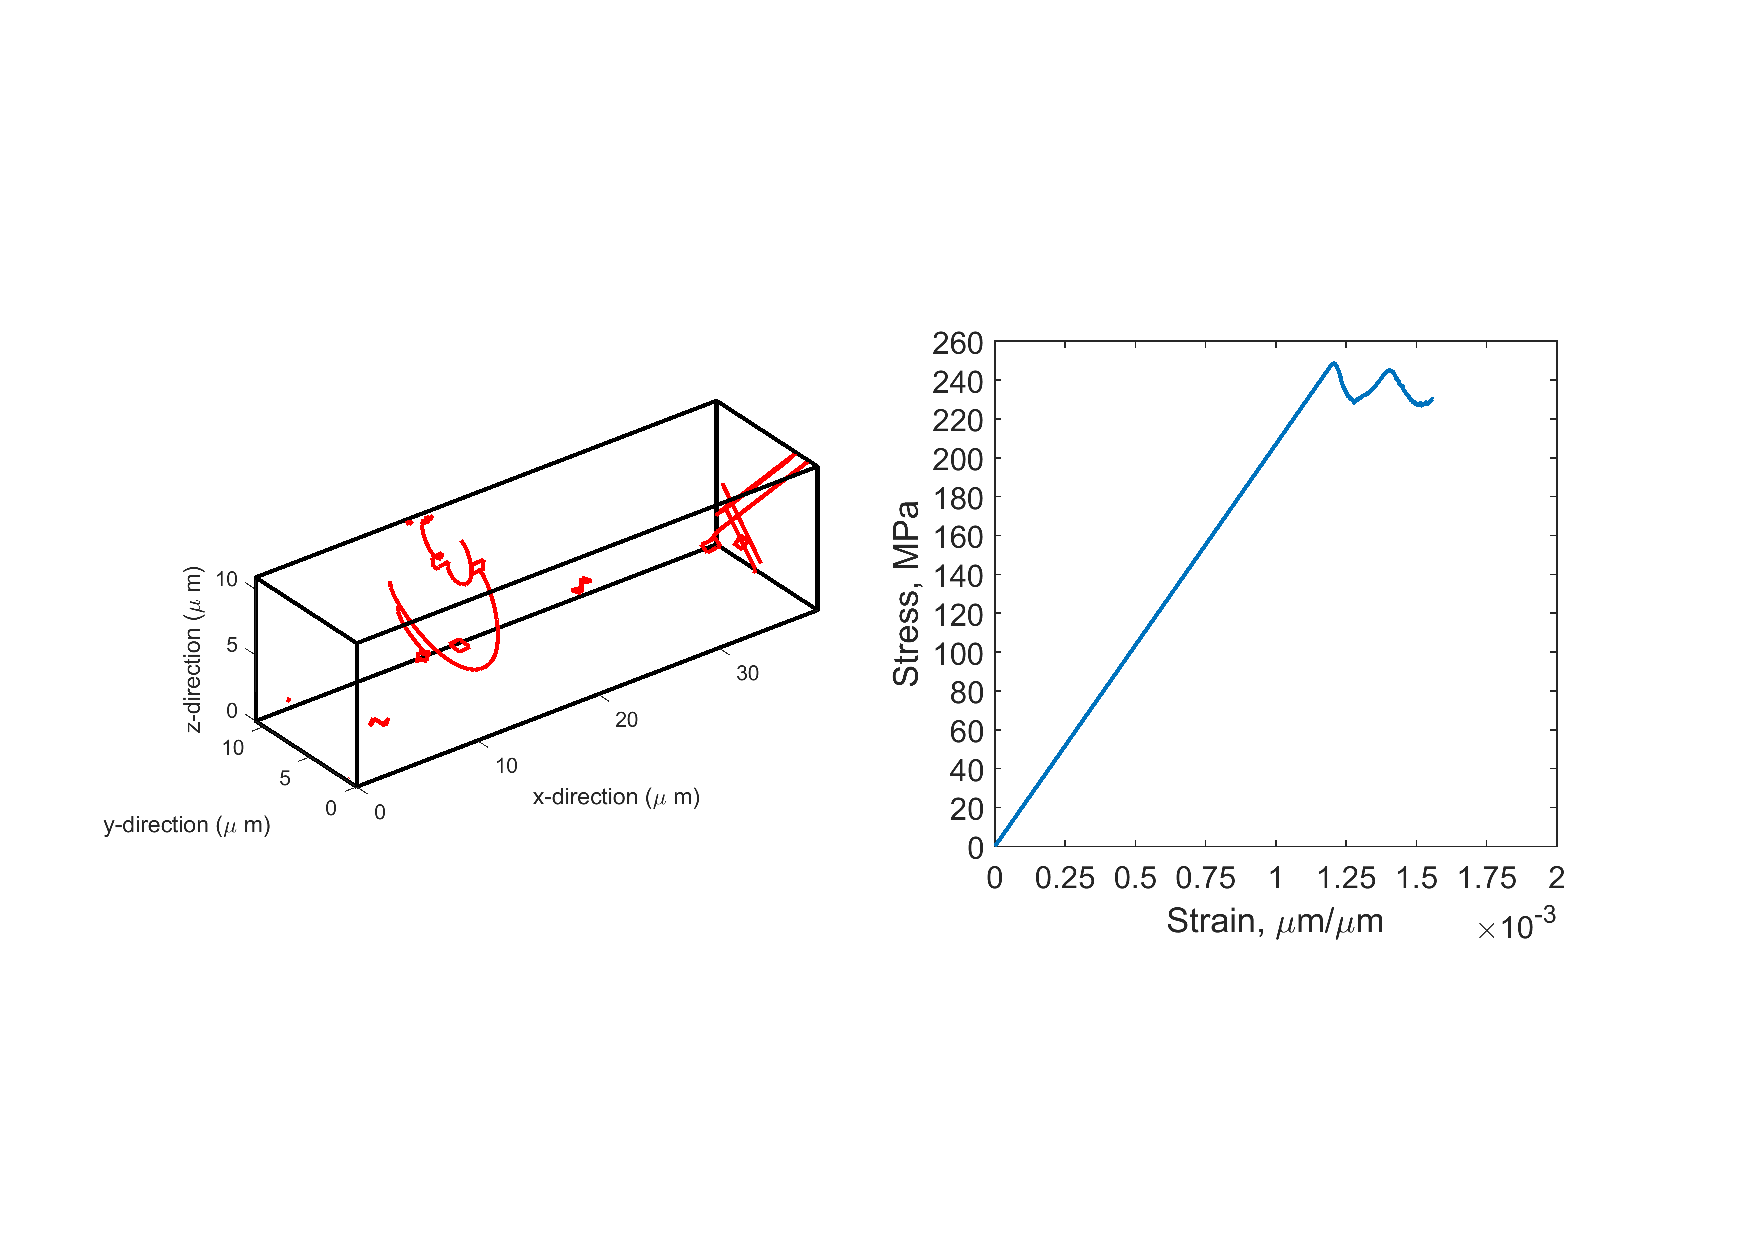
\includegraphics[trim={1.75cm 5cm 2.5cm 5.5cm},clip,width=\linewidth]{../data/11-Mar-2021_8_tensile_ni_100_120000.pdf}
        \caption{Upward slope.}
    \end{subfigure}
    \caption[Dislocation structure with corresponding load displacement curves of tensile loading in $\langle 1\, 0\, 0 \rangle$.]{Dislocation structure with corresponding load displacement curves of tensile loading in $\langle 1\, 0\, 0 \rangle$. Corresponds to (a) in \cref{sf:Ni100_DDD}.}
    \label{f:Ni100_bumps}
\end{figure}

On the other hand, the $\langle 1\, 1\, 0 \rangle$ loading direction does not exhibit such large differences in internal dislocation length, and therefore its stress-strain curve is not as bumpy. This can be seen in \cref{f:Ni110_bumps}, which corresponds to simulation (a) from \cref{sf:Ni110_DDD}.
\begin{figure}
    \centering
    \begin{subfigure}[t]{\linewidth}
        \centering
        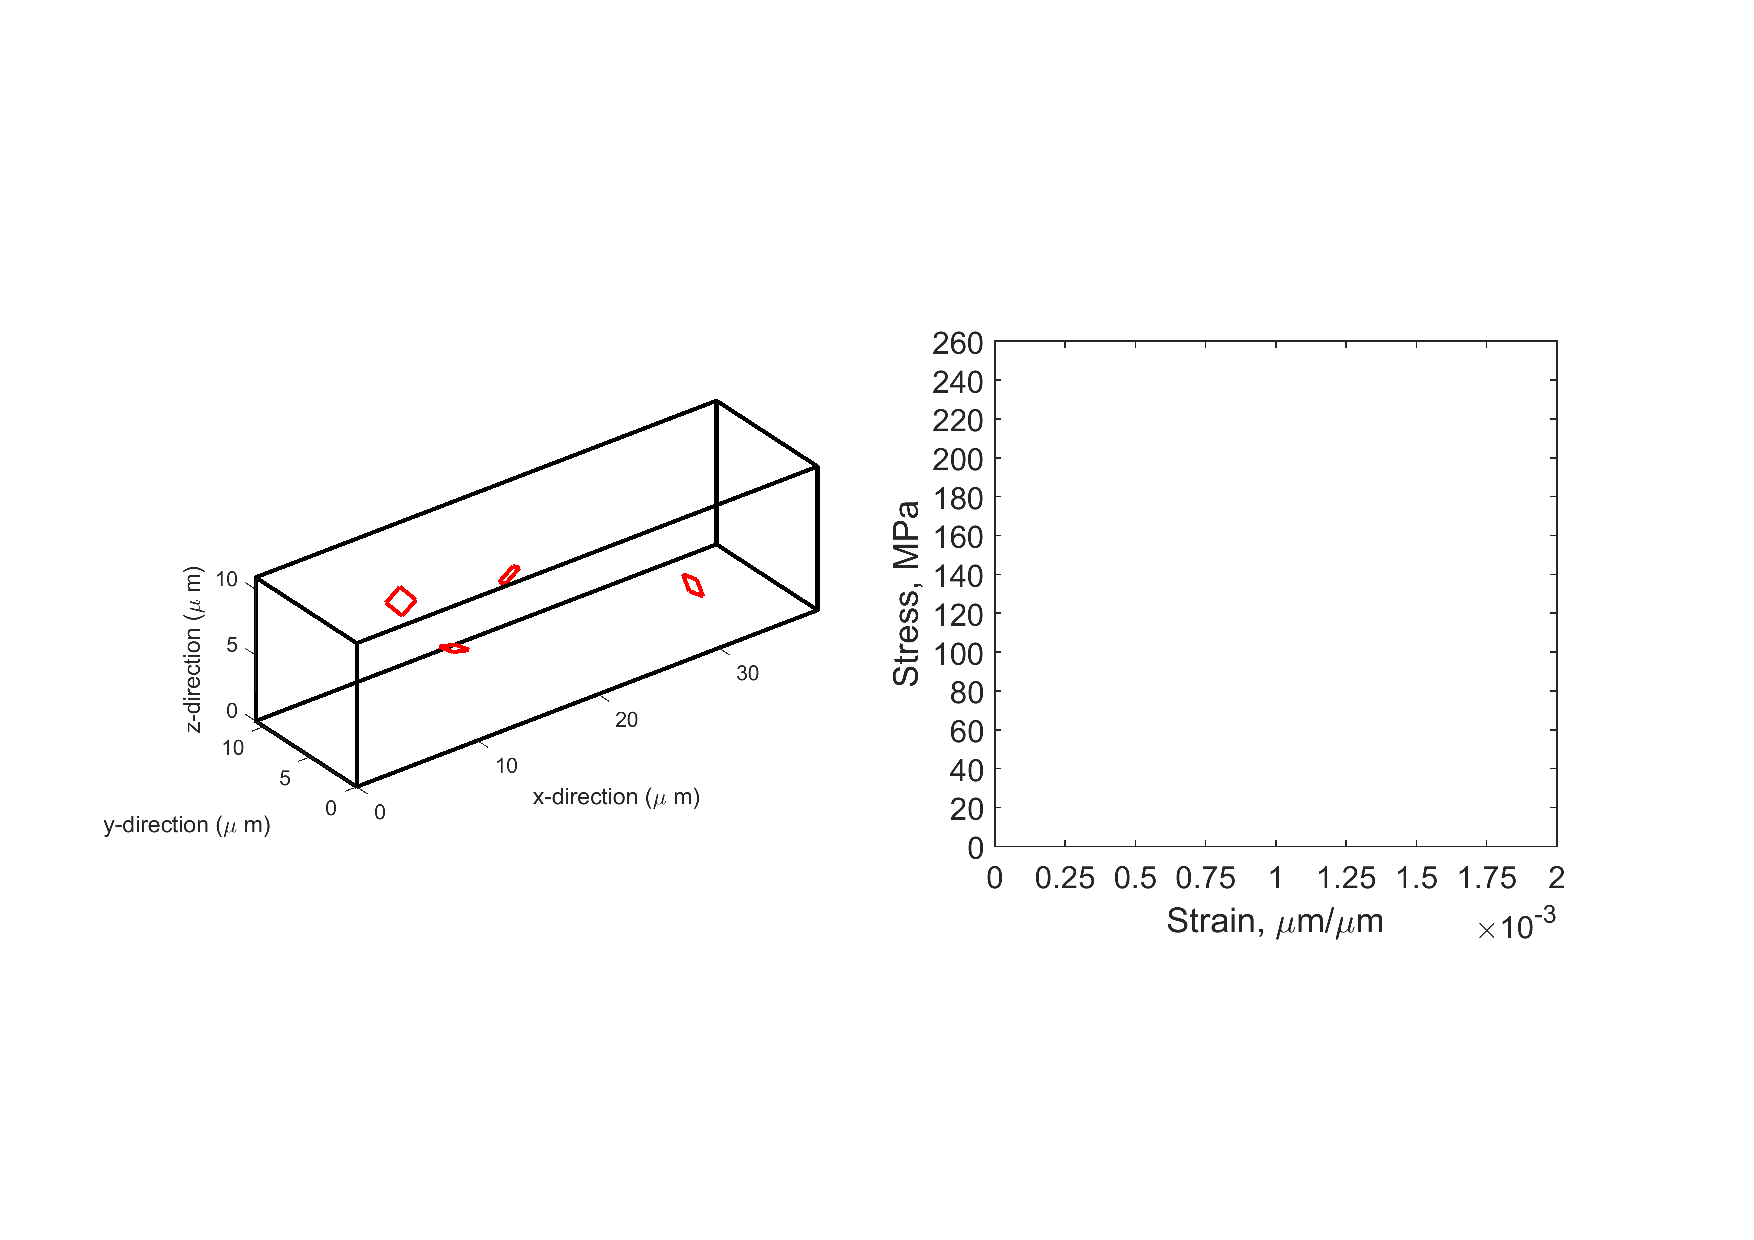
\includegraphics[trim={1.75cm 5cm 2.5cm 5.5cm},clip,width=\linewidth]{../data/16-Mar-2021_4_tensile_ni_110_0.pdf}
        \caption{Initial structure.}
    \end{subfigure}

    \begin{subfigure}[t]{\linewidth}
        \centering
        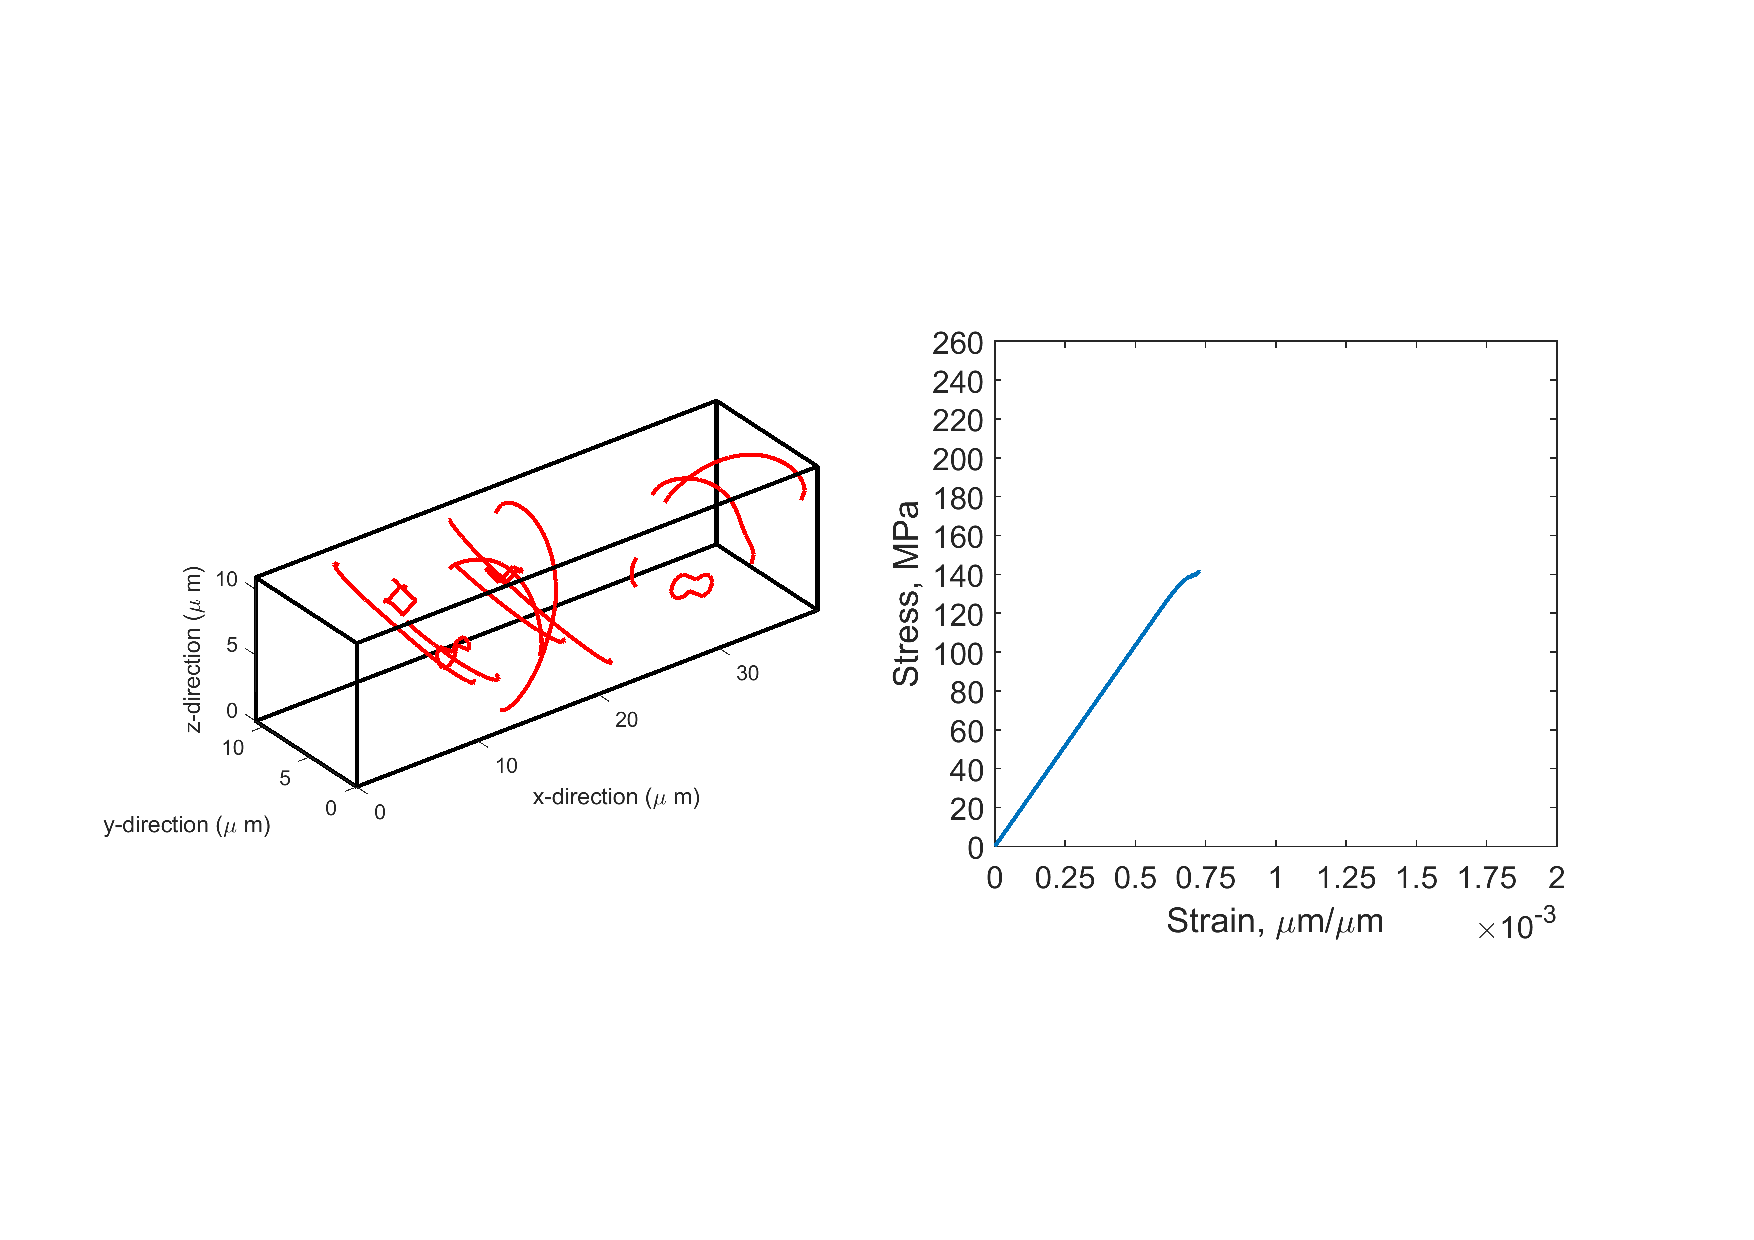
\includegraphics[trim={1.75cm 5cm 2.5cm 5.5cm},clip,width=\linewidth]{../data/16-Mar-2021_4_tensile_ni_110_5400.pdf}
        \caption{Start of plasticity.}
    \end{subfigure}

    \begin{subfigure}[t]{\linewidth}
        \centering
        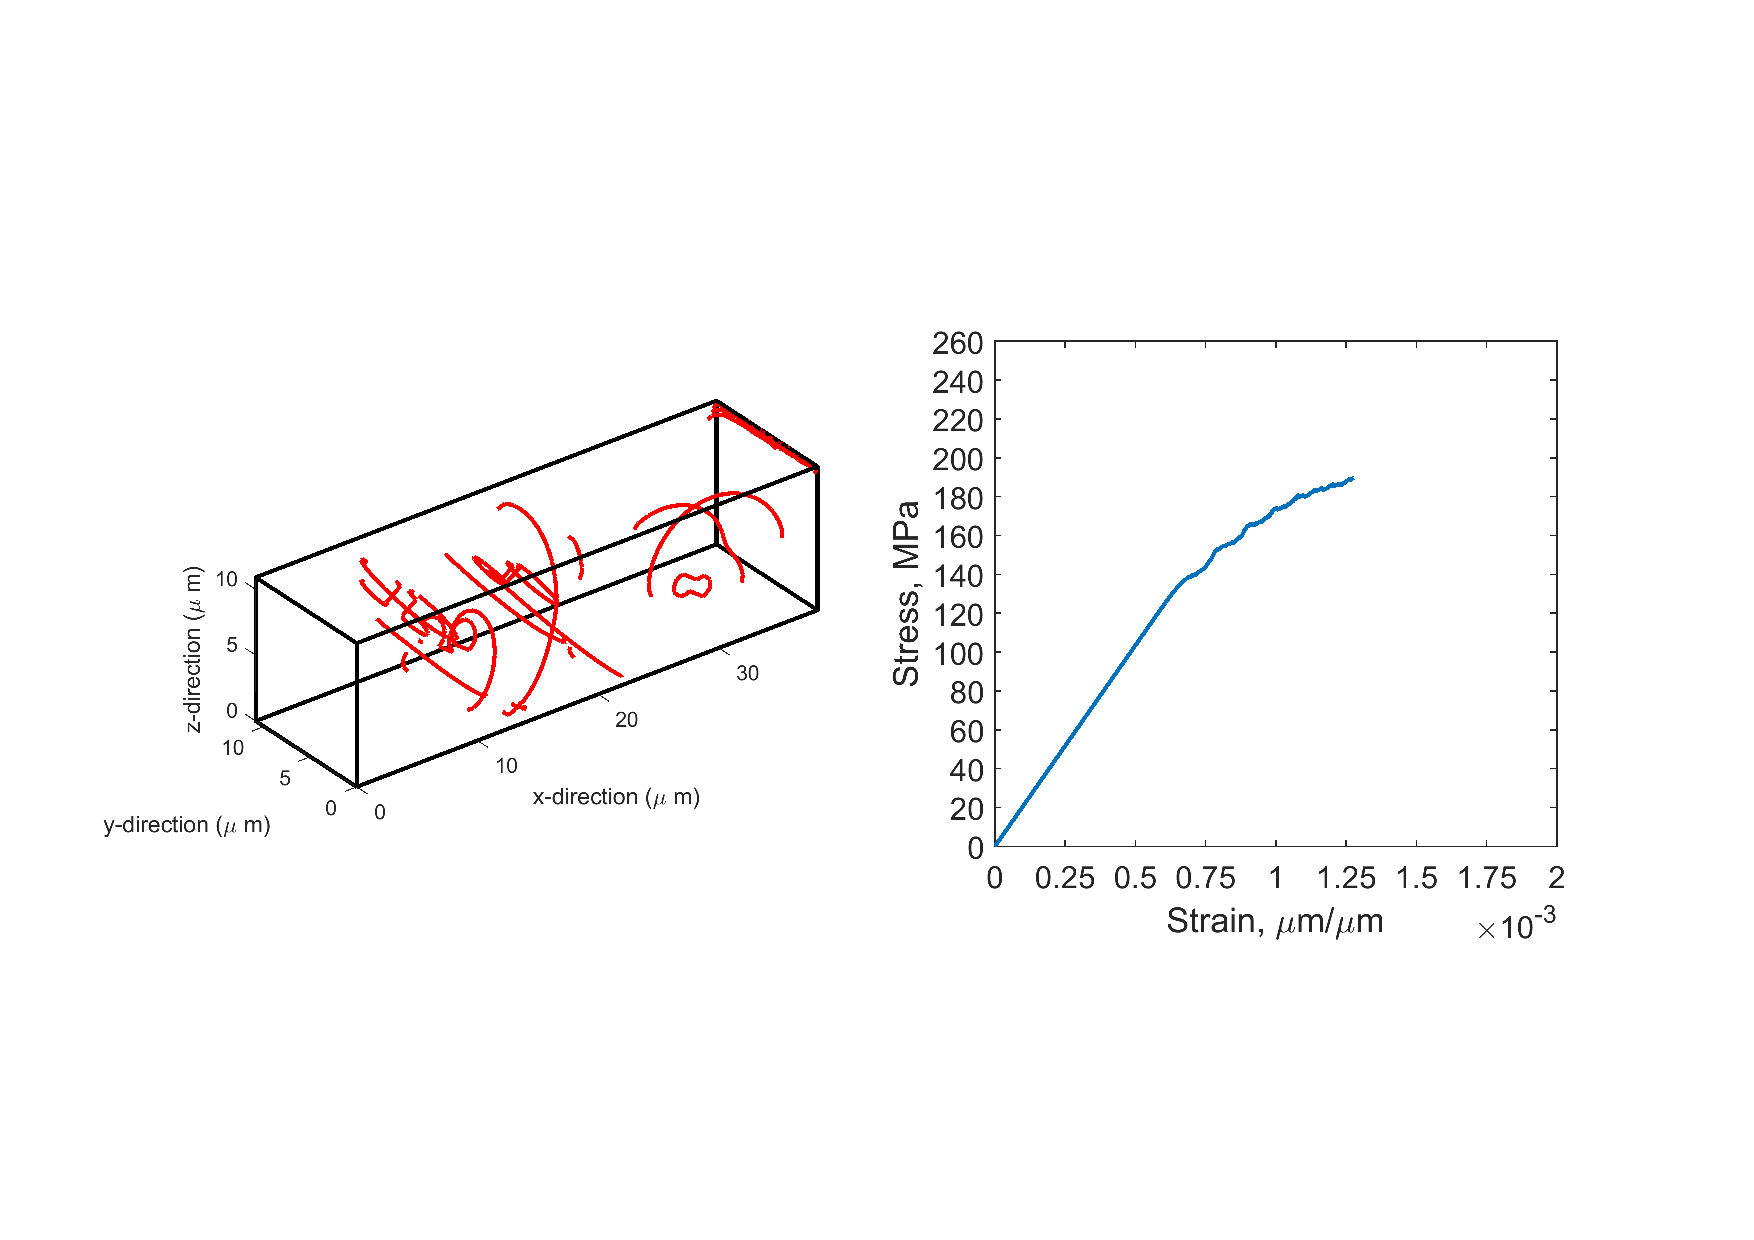
\includegraphics[trim={1.75cm 5cm 2.5cm 5.5cm},clip,width=\linewidth]{../data/16-Mar-2021_4_tensile_ni_110_225000.pdf}
        \caption{End of simulation.}
    \end{subfigure}
    \caption[Dislocation structure with corresponding load displacement curves of tensile loading in $\langle 1\, 1\, 0 \rangle$.]{Dislocation structure with corresponding load displacement curves of tensile loading in $\langle 1\, 1\, 0 \rangle$. Corresponds to (b) in \cref{sf:Ni110_DDD}.}
    \label{f:Ni110_bumps}
\end{figure}

We have also produced \texttt{mp4} videos of all our useable simulations. These behaviours can be confirmed by watching them. The videos are found in the following link \href{https://github.com/dcelisgarza/DPhil_Thesis/tree/master/data}{https://github.com/dcelisgarza/DPhil\_Thesis/tree/master/data}.

Curves (a) and (b) in \cref{sf:Ni100_DDD} represent the same initial conditions, except for the fact that (a) uses analytic tractions, and (b) numeric ones (see \cref{c:tractions}). At a glance, it is clear the numeric tractions did a very good job at reproducing the load displacement curve, until its curve started diverging from the analytic tractions quite significantly. A comparison of the aforementioned videos will make the chaotic nature of dislocation dynamics quite clear. The structures produced from both methods diverge very quickly, though the load displacement curve does diverge much not change until later.

In this case, the numeric tractions managed to get further than the analytic ones, this is not always true. Moreover, the numeric tractions consistently yield higher stresses as simulations advance, regardless of loading conditions. With an FCC structure, uniform strain, and few sources, the consequences of this aren't immediately obvious. However, when cross-slip is allowed like in a BCC mobility law, or when the strain is not uniform such as in nanoindentation or cantilever bending, the numeric instability of the numeric tractions is often problematic as it tends to cause more cross-slip---and therefore more topological operations---which can dramatically slow simulations down. As mentioned in \cref{c:topology,c:tractions}, we have found the analytic tractions to be much more robust and reliable in comparison, so the recommendation is to use them if available.

We cannot compare exactly equivalent points in the simulations using numeric vs analytic tractions because the integrator is adaptive, but we can at least try to get as close as possible. \Cref{f:analyticNumericStruct} shows a few roughly equivalent points in strain, yet they all have visibly different dislocation structures, except for the initial distribution.
\begin{figure}
    \centering
    \begin{subfigure}[t]{0.45\linewidth}
        \centering
        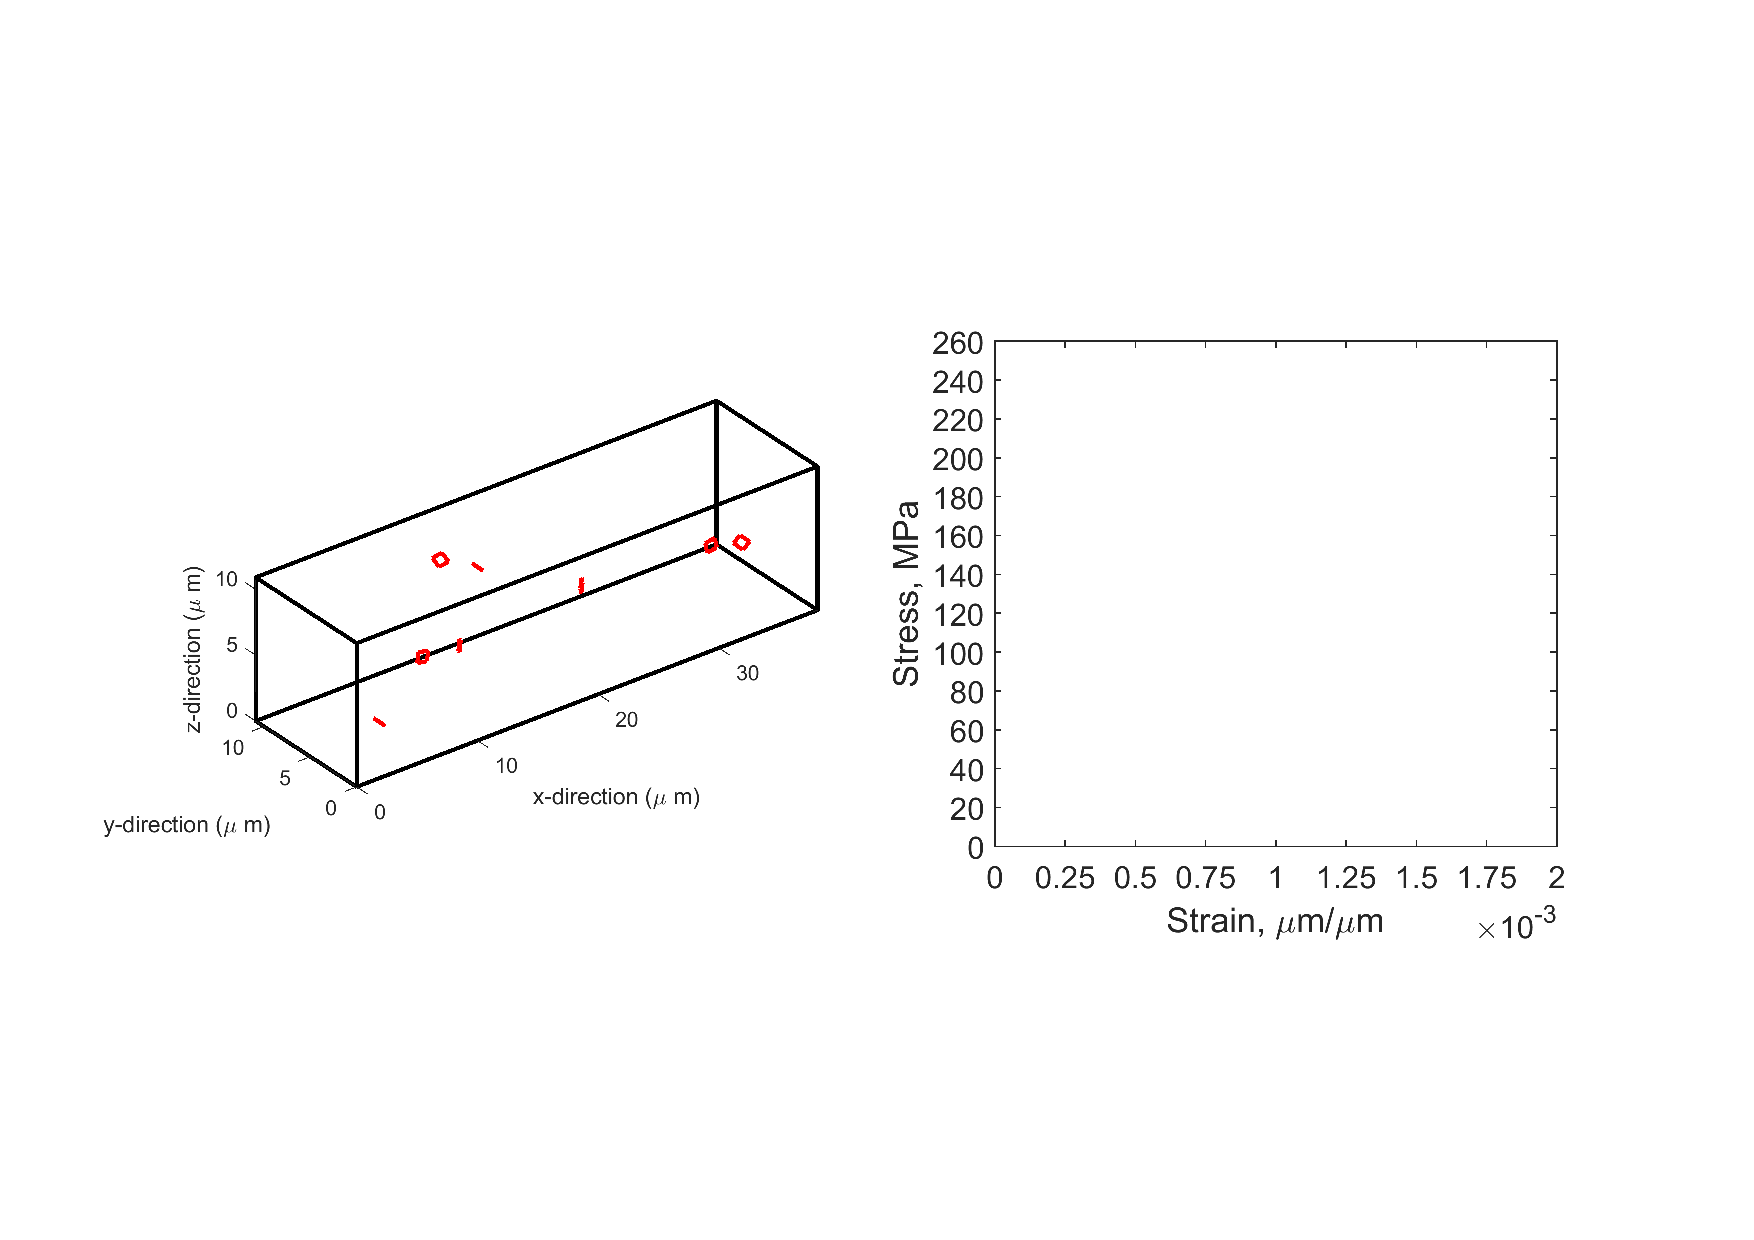
\includegraphics[trim={1.75cm 6.75cm 15.75cm 6.75cm},clip,width=\linewidth]{../data/11-Mar-2021_numT_8_tensile_ni_100_0.pdf}
        \caption{Numeric tractions at 0\% strain.}
    \end{subfigure}
    ~
    \begin{subfigure}[t]{0.45\linewidth}
        \centering
        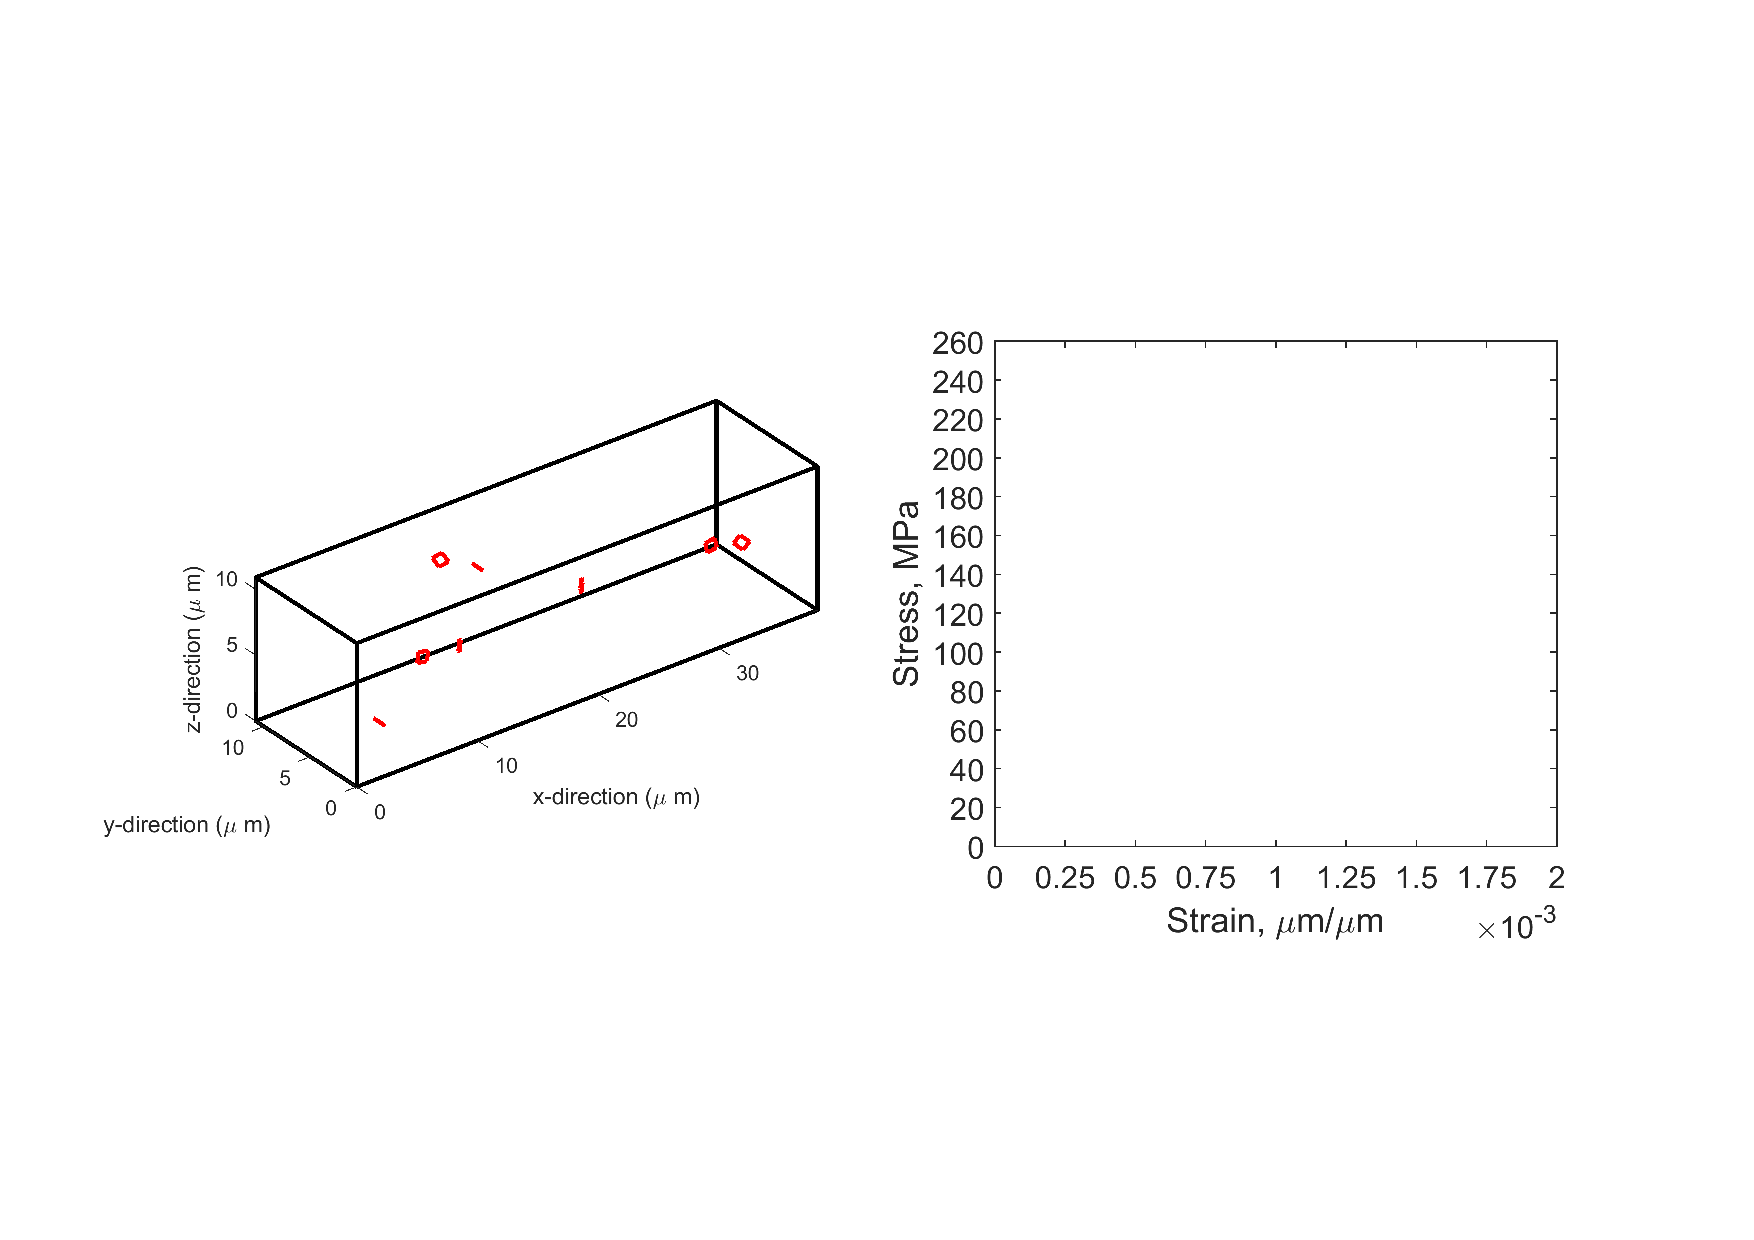
\includegraphics[trim={1.75cm 6.75cm 15.75cm 6.75cm},clip,width=\linewidth]{../data/11-Mar-2021_8_tensile_ni_100_0.pdf}
        \caption{Analytic tractions at 0\% strain.}
    \end{subfigure}

    \begin{subfigure}[t]{0.45\linewidth}
        \centering
        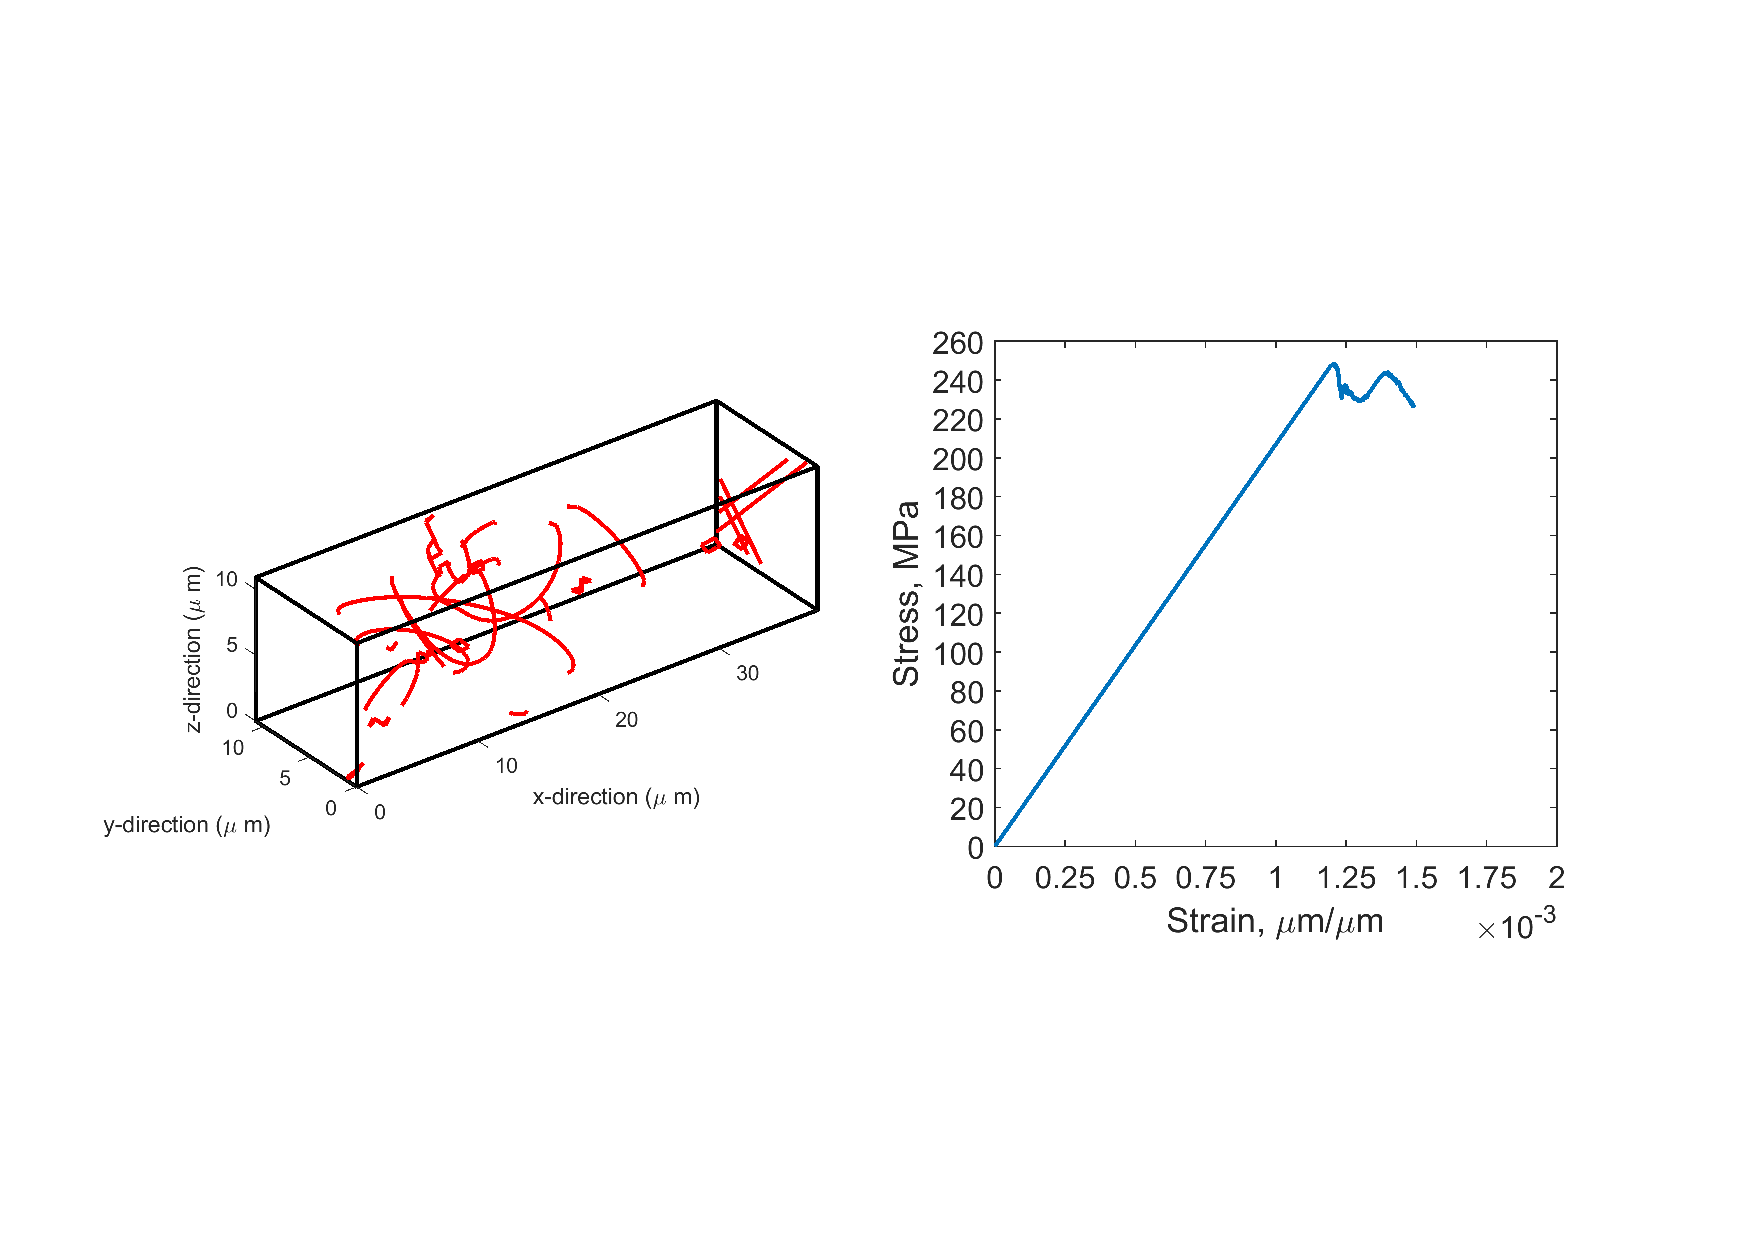
\includegraphics[trim={1.75cm 6.75cm 15.75cm 6.75cm},clip,width=\linewidth]{../data/11-Mar-2021_numT_8_tensile_ni_100_81600.pdf}
        \caption{Numeric tractions at 0.1491\% strain.}
    \end{subfigure}
    ~
    \begin{subfigure}[t]{0.45\linewidth}
        \centering
        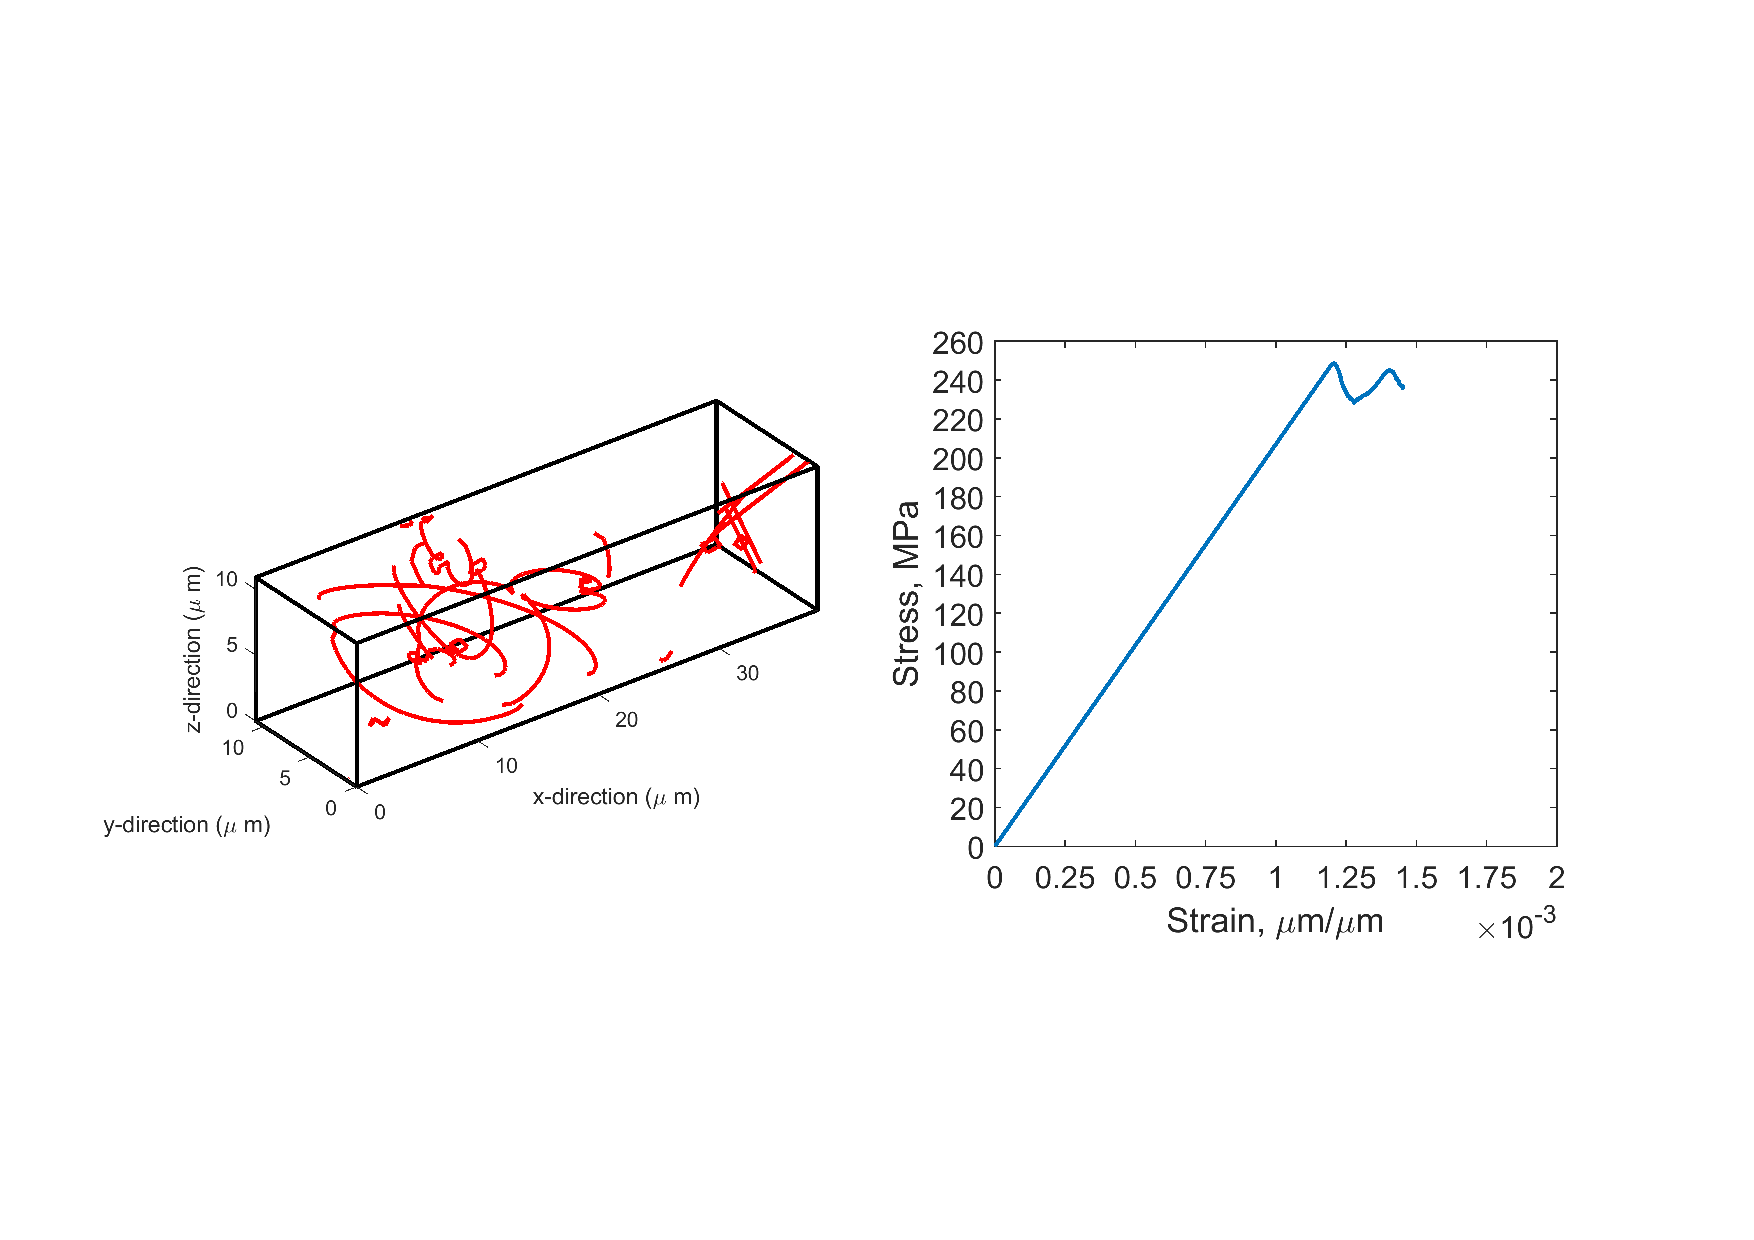
\includegraphics[trim={1.75cm 6.75cm 15.75cm 6.75cm},clip,width=\linewidth]{../data/11-Mar-2021_8_tensile_ni_100_60000.pdf}
        \caption{Analytic tractions at 0.1454\% strain.}
    \end{subfigure}

    \begin{subfigure}[t]{0.45\linewidth}
        \centering
        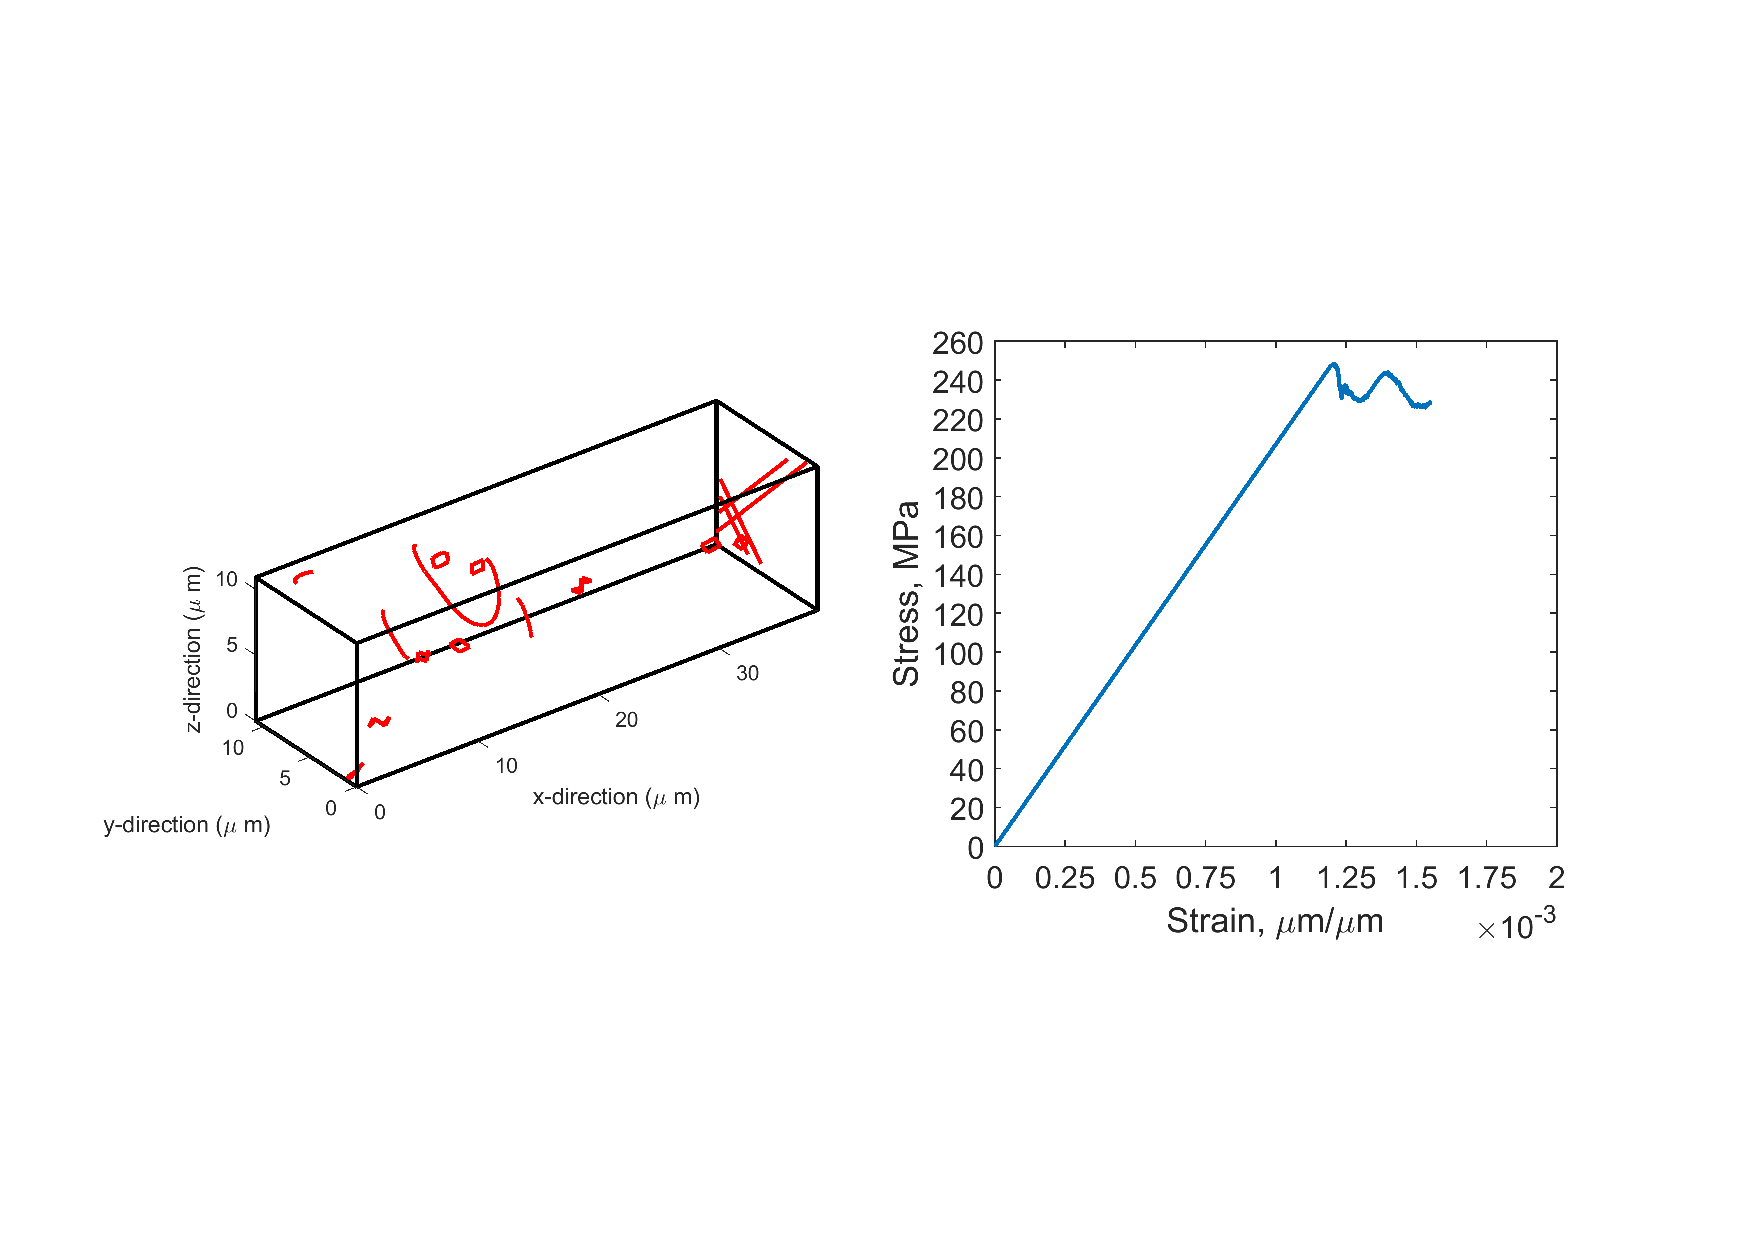
\includegraphics[trim={1.75cm 6.75cm 15.75cm 6.75cm},clip,width=\linewidth]{../data/11-Mar-2021_numT_8_tensile_ni_100_98400.pdf}
        \caption{Numeric tractions at 0.1552\% strain.}
    \end{subfigure}
    ~
    \begin{subfigure}[t]{0.45\linewidth}
        \centering
        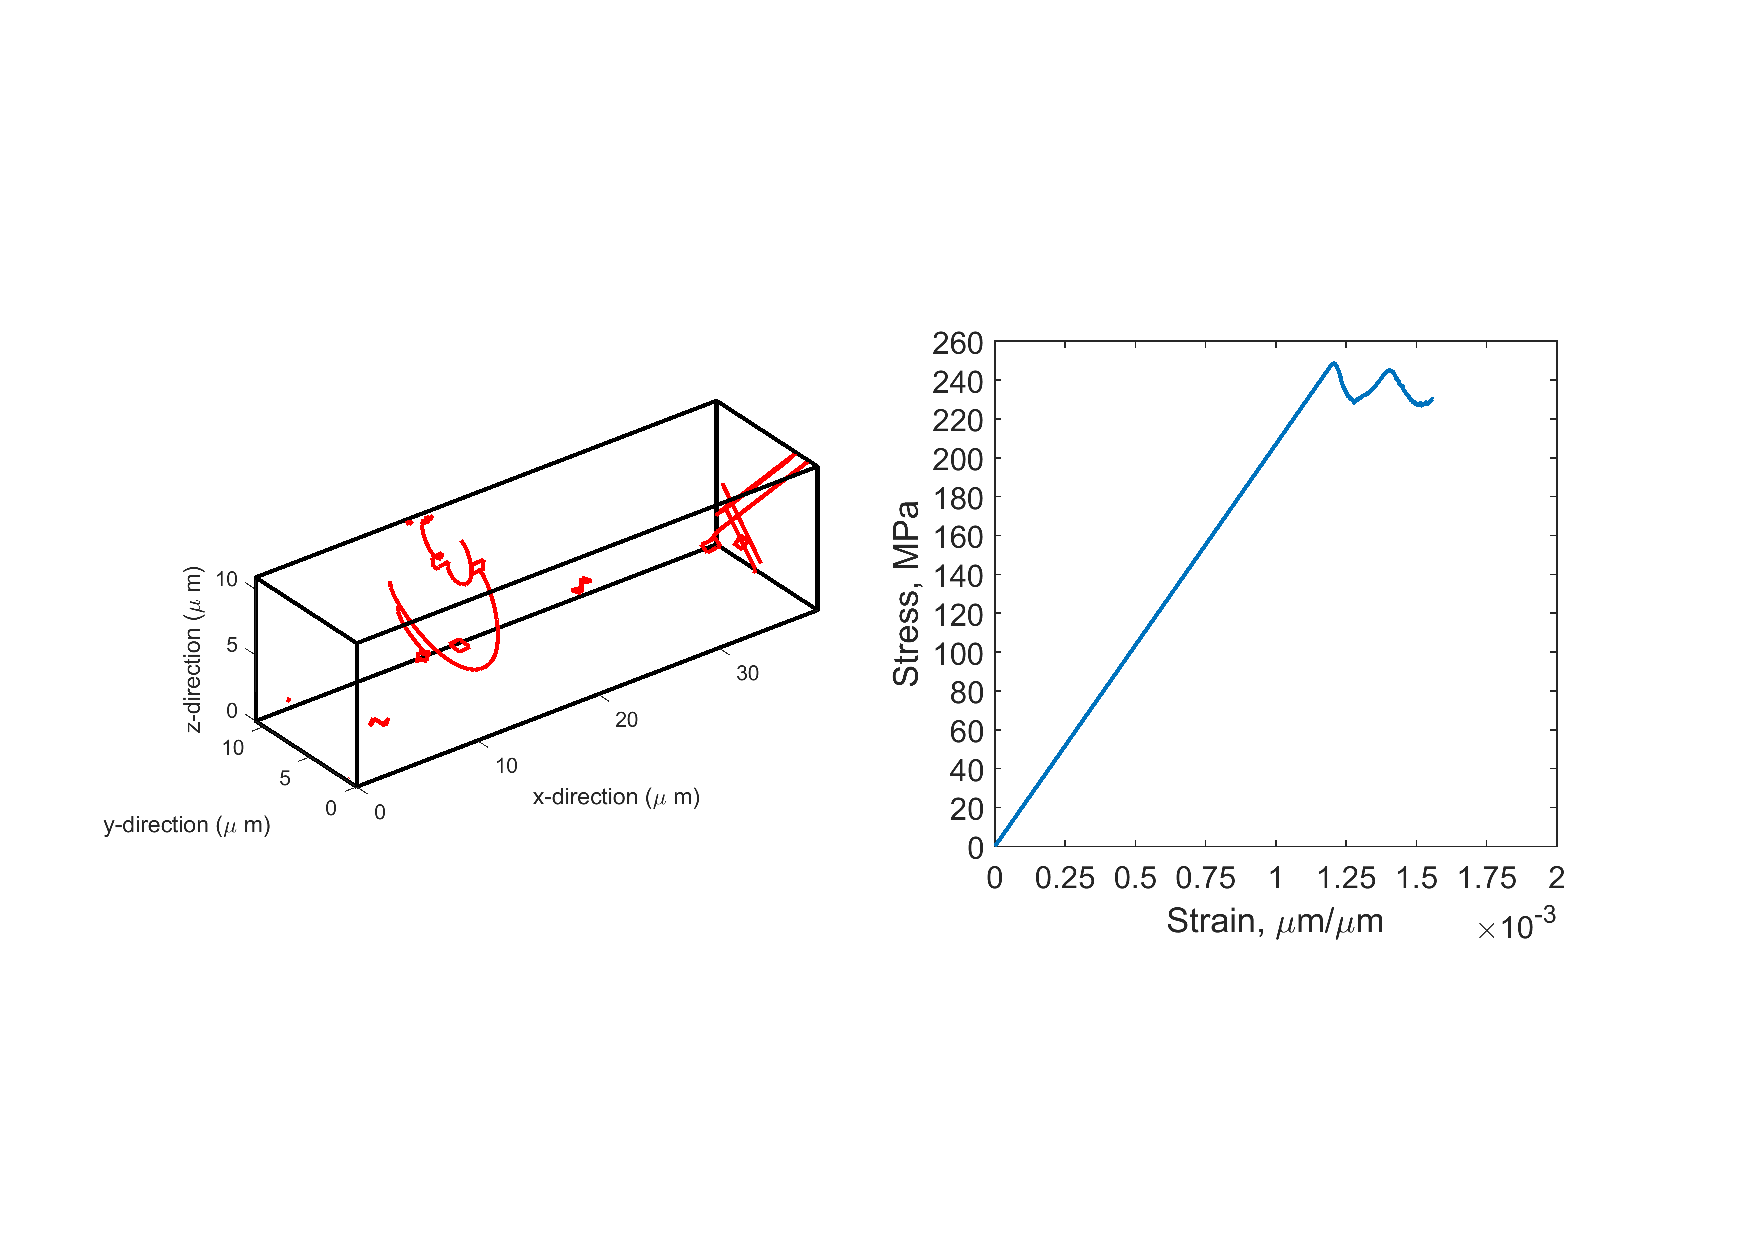
\includegraphics[trim={1.75cm 6.75cm 15.75cm 6.75cm},clip,width=\linewidth]{../data/11-Mar-2021_8_tensile_ni_100_120000.pdf}
        \caption{Analytic tractions at 0.1558\% strain.}
    \end{subfigure}
    \caption[Differences in dislocation structures when using numeric or analytic tractions with the same initial conditions.]{Differences in dislocation structures when using numeric or analytic tractions with the same initial conditions. Tensile loading in $\langle 1\, 0\, 0 \rangle$, analytic and numeric tractions respectively correspond to curves (a) and (b) of \cref{sf:Ni100_DDD}.}
    \label{f:analyticNumericStruct}
\end{figure}

The final aspect of reproducing experimental results with dislocation plasticity is to see what the slip steps look like. Again, given the time scales and small strains we can simulate with dislocation plasticity, we will not see slip steps that are as large as those experimentally observed. Each exited dislocation with Burgers vector $\vec{b}$ will create a corresponding slip step with the same vector and magnitude. As more loops generated by the FR source keep exiting the domain, the slip step grows by $b$ each time one of them exits the surface. Using the dislocation-induced displacements described in \cite{bromage2018calculating}, we plot the slip steps at the final states of our simulations in \cref{f:slipSteps}.
\begin{figure}
    \centering
    \begin{subfigure}[t]{0.45\linewidth}
        \centering
        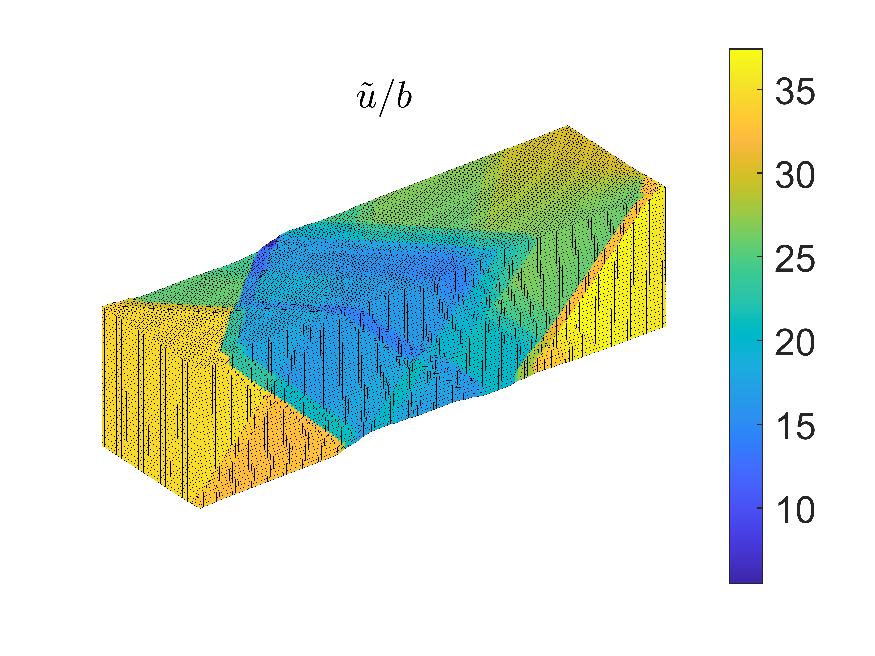
\includegraphics[width=\linewidth]{../data/11-Mar-2021_8_tensile_ni_100_196800_disp.pdf}
        \caption{Tensile loading in $\langle 1\, 0\, 0 \rangle$. Corresponds to (a) in \cref{sf:Ni100_DDD} (analytic tractions).}
        \label{sf:Ni100a_disp}
    \end{subfigure}
    ~
    \begin{subfigure}[t]{0.45\linewidth}
        \centering
        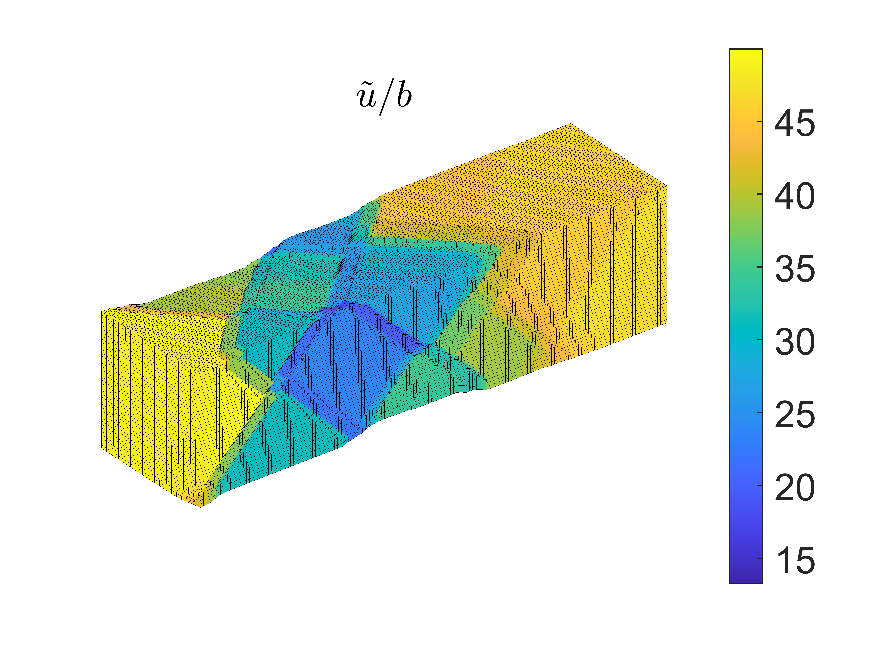
\includegraphics[width=\linewidth]{../data/11-Mar-2021_numT_8_tensile_ni_100_168600_disp.pdf}
        \caption{Tensile loading in $\langle 1\, 0\, 0 \rangle$. Corresponds to (b) in \cref{sf:Ni100_DDD} (numeric tractions).}
        \label{sf:Ni100aN_disp}
    \end{subfigure}

    \begin{subfigure}[t]{0.45\linewidth}
        \centering
        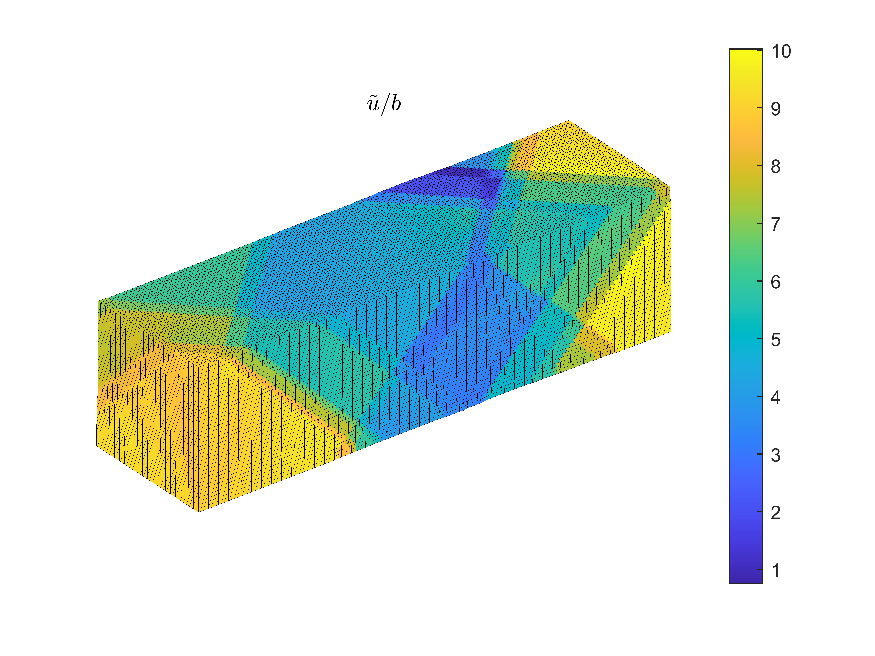
\includegraphics[width=\linewidth]{../data/16-Mar-2021_8_tensile_ni_100_214400_disp.pdf}
        \caption{Tensile loading in $\langle 1\, 0\, 0 \rangle$. Corresponds to (c) in \cref{sf:Ni100_DDD}.}
        \label{sf:Ni100b_disp}
    \end{subfigure}

    \begin{subfigure}[t]{0.45\linewidth}
        \centering
        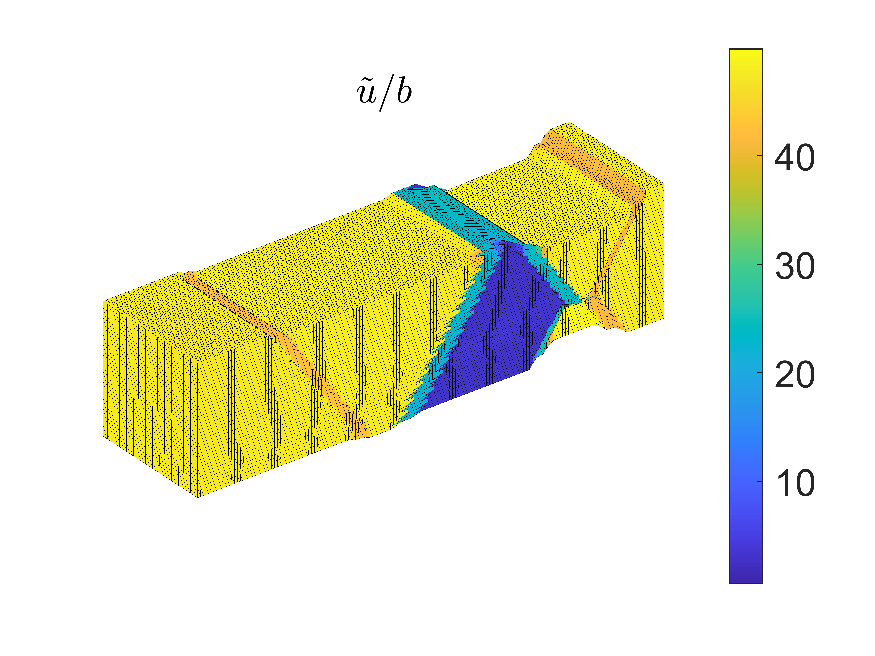
\includegraphics[width=\linewidth]{../data/11-Mar-2021_4_tensile_ni_110_205600_disp.pdf}
        \caption{Tensile loading in $\langle 1\, 1\, 0 \rangle$. Corresponds to (a) in \cref{sf:Ni110_DDD}.}
        \label{sf:Ni110a_disp}
    \end{subfigure}
    ~
    \begin{subfigure}[t]{0.45\linewidth}
        \centering
        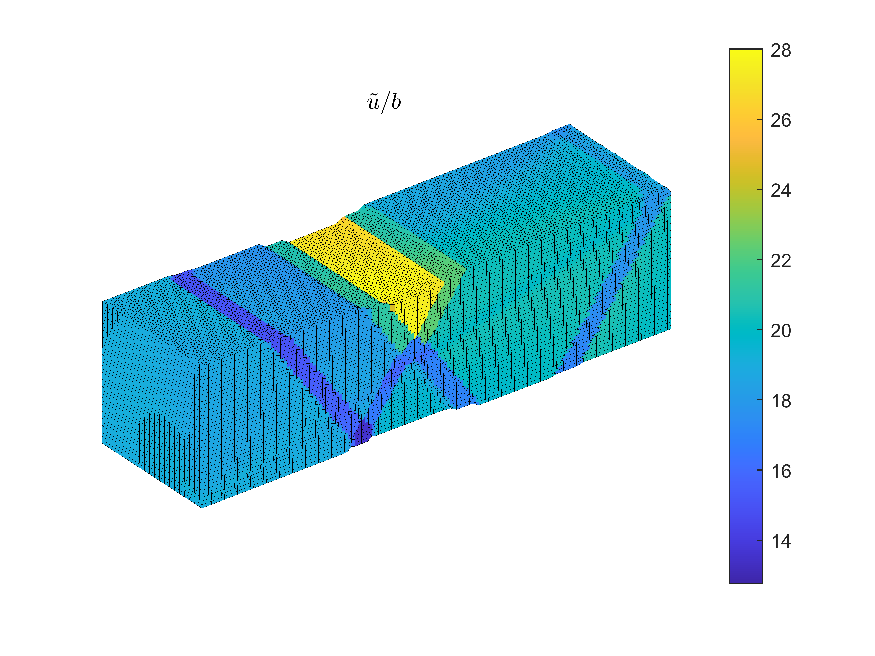
\includegraphics[width=\linewidth]{../data/16-Mar-2021_4_tensile_ni_110_225000_disp.pdf}
        \caption{Tensile loading in $\langle 1\, 1\, 0 \rangle$. Corresponds to (b) in \cref{sf:Ni110_DDD}.}
        \label{sf:Ni110b_disp}
    \end{subfigure}
    \caption[Slip steps normalised to Burgers vector magnitude for the final states of tensile loading simulations.]{Slip steps normalised to Burgers vector magnitude for the final states of tensile loading simulations. The displacements are scaled $100\times$ for display purposes, the colour bars are not scaled.}
    \label{f:slipSteps}
\end{figure}

The first thing of note is the fact that the slip steps of simulations with higher strain present larger slip steps than other simulations of the same system. The second thing is that for the $\langle 1\, 0\, 0 \rangle$ loading direction, the numeric tractions (\cref{sf:Ni100aN_disp}) produce one slip step that is much larger than the corresponding one in (\cref{sf:Ni100a_disp}). This is not an artifact of the fact that the numeric tractions achieved a larger strain. In reality, it is due to the increased activity of the source closest to the origin compared to the analytic counterpart. This is readily observed in the aformentioned videos.

Unfortunately we do not have experimental imaging data corresponding to the $\langle 1\, 1\, 0 \rangle$ loading direction, but the slip step patterns of \cref{sf:Ni100a_disp,sf:Ni100aN_disp,sf:Ni100b_disp} are \emph{very} similar to those observed in \cref{f:Ni100_disp}, including the criss-crossing of slip steps. Granted, the slip steps from the simulations are not remotely of the same magnitude; nor are they in the same places; and likely not with the same distribution as it appears the real dislocations are mostly located near the ends of the pillar, where it starts curving into the bulk; but they are extremely similar. That said, in all plots of \cref{f:slipSteps}, except \cref{sf:Ni110b_disp}, the largest slip steps are also concentrated near the ends of the simulation domain. One could even argue \cref{f:slipSteps} shows the beginning of necking, as observed in \cref{sf:necking}.
\begin{figure}
    \centering
    \begin{subfigure}[t]{0.45\linewidth}
        \centering
        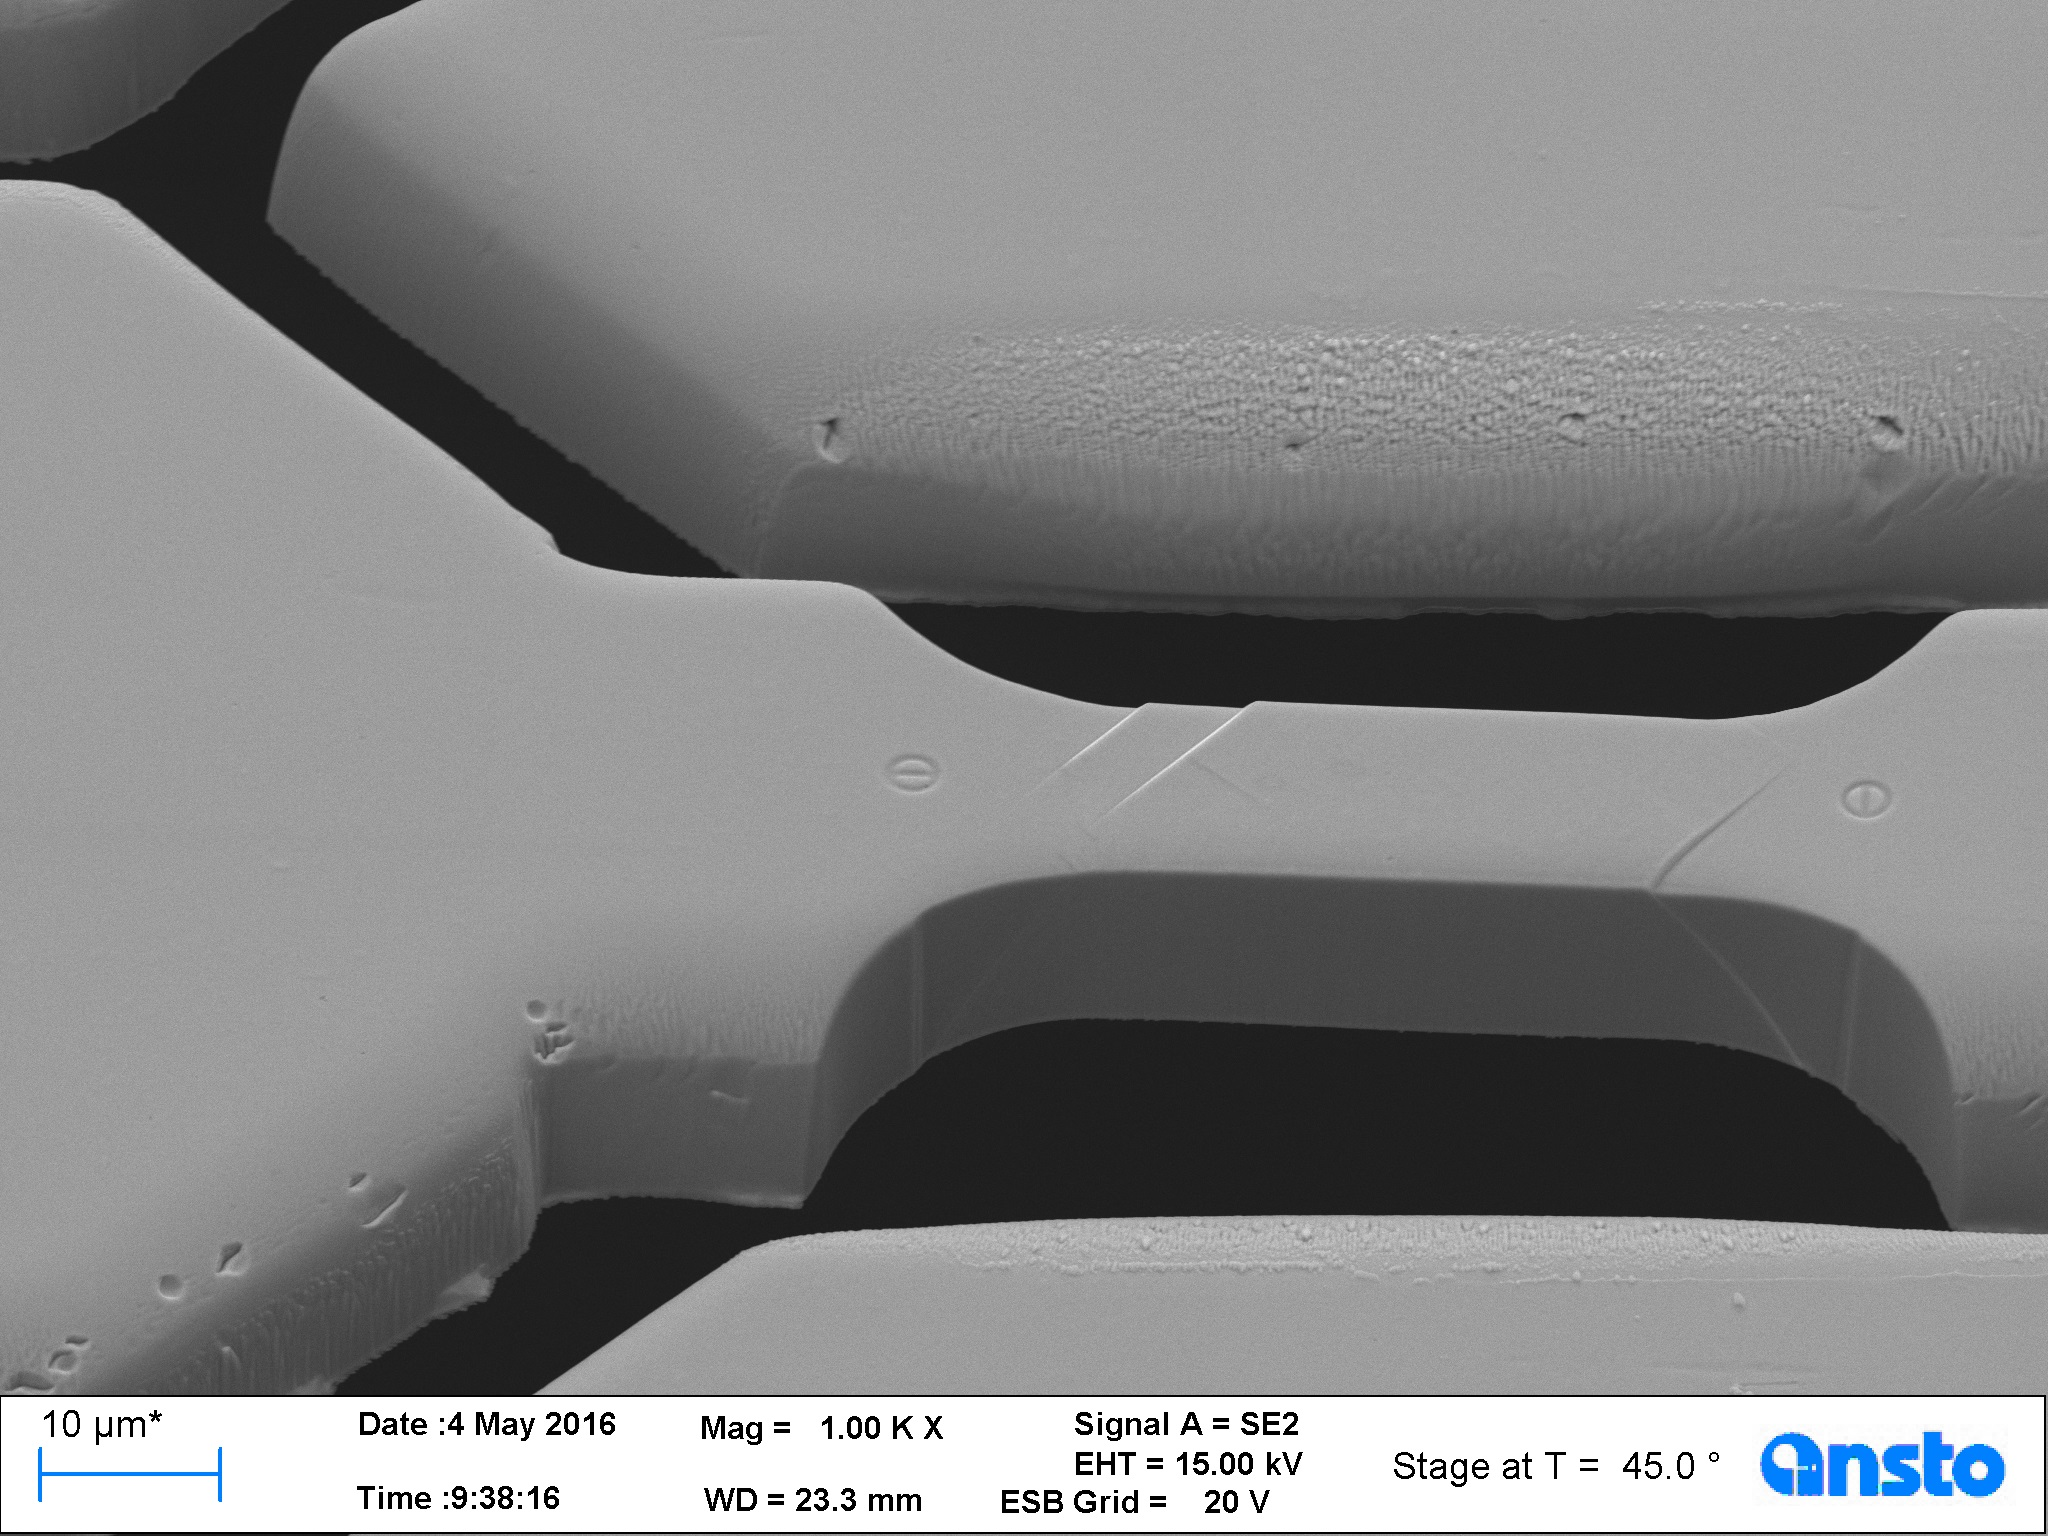
\includegraphics[width=\linewidth]{../data/Ni016.jpg}
        \caption{}
    \end{subfigure}
    ~
    \begin{subfigure}[t]{0.45\linewidth}
        \centering
        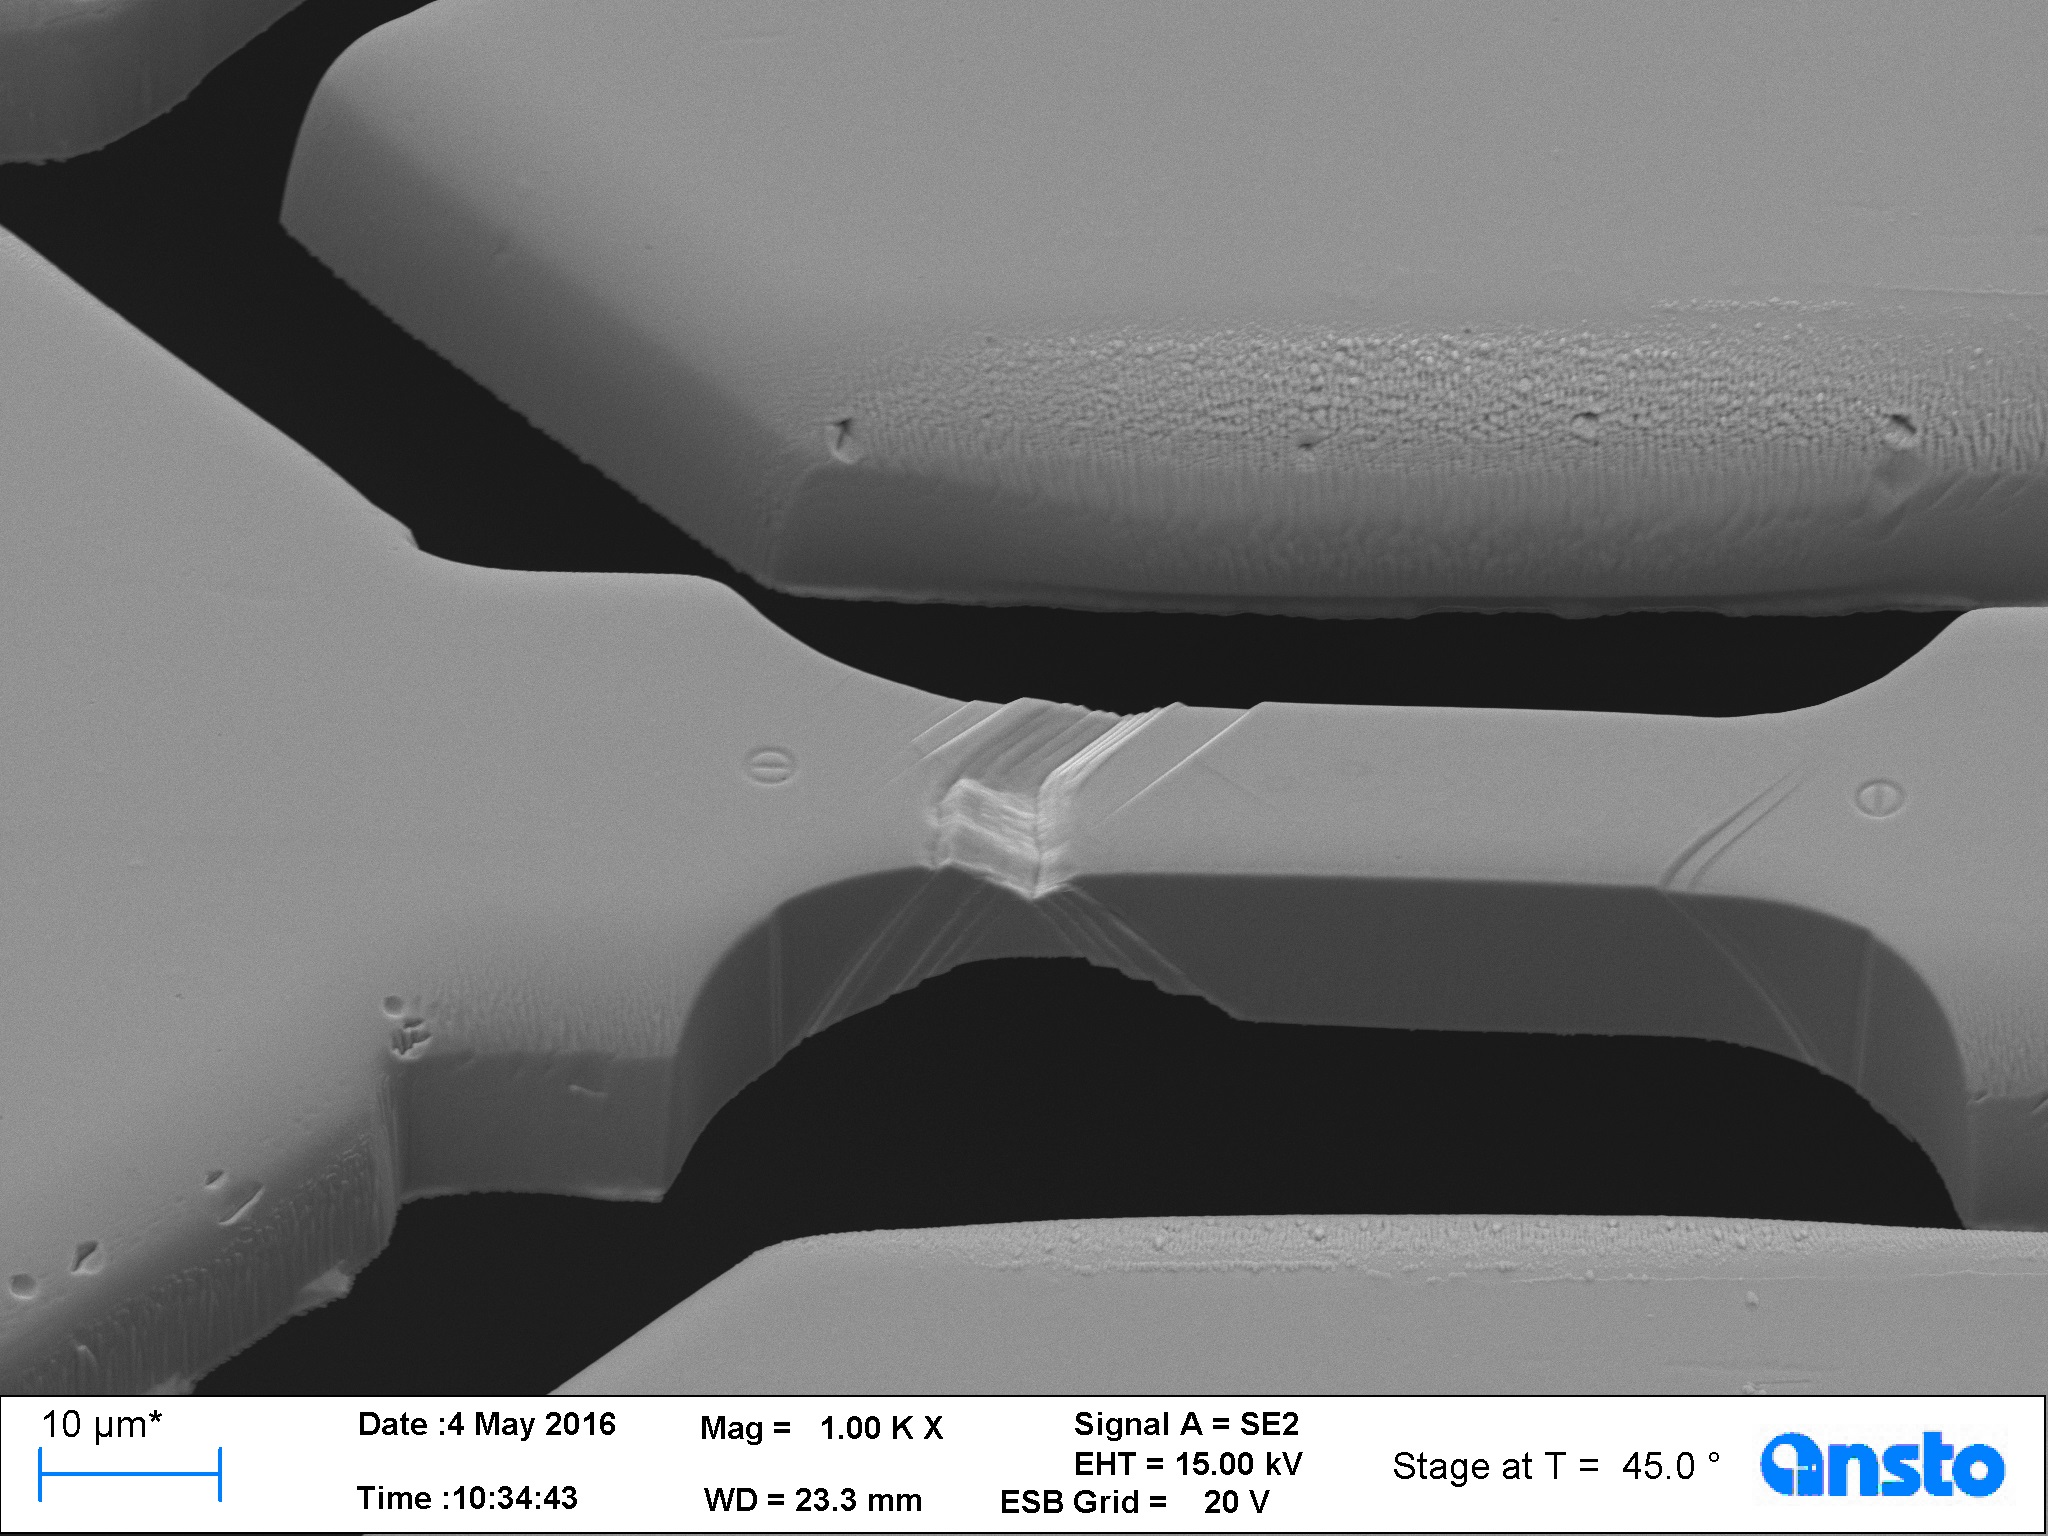
\includegraphics[width=\linewidth]{../data/Ni023.jpg}
        \caption{}
        \label{sf:necking}
    \end{subfigure}
    \caption[SEM images of tensile test in $\langle 1\, 0\, 0 \rangle$.]{SEM images of tensile test in $\langle 1\, 0\, 0 \rangle$. (a) shows slip steps forming and (b) shows necking as the strain increases.}
    \label{f:Ni100_disp}
\end{figure}

With the resolution of the SEM images, it is hard to tell exactly how many slip steps there are in the experimental measurements. Furthermore, the simulations have not reached anywhere near the strains of the experiments. However, it is clearly evident that we can reproduce the phenomenology behind experimental observations in very fine detail thanks to dislocation plasticity, at least at small strains.

\section{Conclusions}
\label{s:concSim}

The point of dislocation plasticity simulations is to provide insight as to the mechanisms behind plasticity. Even with its limitations to small strains, its strong assumptions, and the necessity for extremely high loading rates, it can offer insight and explain the phenomena we can experimentally observe.

We made some very strong assumptions in \cref{ss:modelSetup} regarding the distribution, size, number and participating slip systems. Obtaining these parameters for things such as micropillars is impossible, one may be able to use a TEM sample as a proxy and make an educated guess from there. However, we have shown that some very simple assumptions with very few sources work remarkably well, at least when the sample is monocrystalline as was the case here. It is hard to extrapolate whether such simple assumptions with so few sources are appropriate for other types of simulations, but there may be some wisdom that can be gleaned from this. Perhaps it is better and more accurate to increase the size of the sources rather than their number, as well as dropping the loading rates as low as practically viable.

We managed to show slip steps and the beginning of necking behaviour that closely follow experimental patterns. We also managed to reproduce the yield stresses for both $\langle 1\, 0\, 0 \rangle$, $\langle 1\, 1\, 0 \rangle$ loading directions, to within experimental variation even when using much larger strain rates. The $\langle 1\, 0\, 0 \rangle$ simulations also showed the ``bumpiness'' of the experimental data, the reasons behind it, as well as how and why it differs from what is observed when loading the $\langle 1\, 1\, 0 \rangle$ direction.

Unfortunately, the spatial and time scales of dislocation plasticity, as well as the practical constraints of time and computational resources did not allow us to reach the same strains as the experiments. So we cannot be sure how the curves will behave going forward. Doubtless the stresses would increase, but would we see the dramatic increases and dips in stresses as the strains increase? The experimental setup is not sensitive enough to probe such small strains, so the simulations can only serve as a bridge between atomic and microscopic scales.

We also only included active slip systems in either loading direction, so the question remains as to how including the inactive systems would affect the results. Our results point towards this assumption being sound, but a future avenue of research would be to include them in future simulations.

The results presented in this chapter are the culmination of meeting the objectives posed for this DPhil, as stated in \cref{s:objectives}. It makes use of the work described in all the other chapters (except for the power dissipation criteria for collision-serparation) and barely scratches at the surface of the remarkable capabilities of dislocation plasticity and EasyDD.
\savearabiccounter
% 3334

